\chapter{Screenshots and Visual Documentation}

This appendix contains screenshots and visual documentation for all five database implementations, demonstrating the practical aspects of each database type.

\section{MongoDB Document Database Screenshots}

The following screenshots demonstrate the MongoDB implementation for the university student management system, showing CRUD operations, complex queries, and aggregation pipelines.

\begin{figure}[H]
\centering
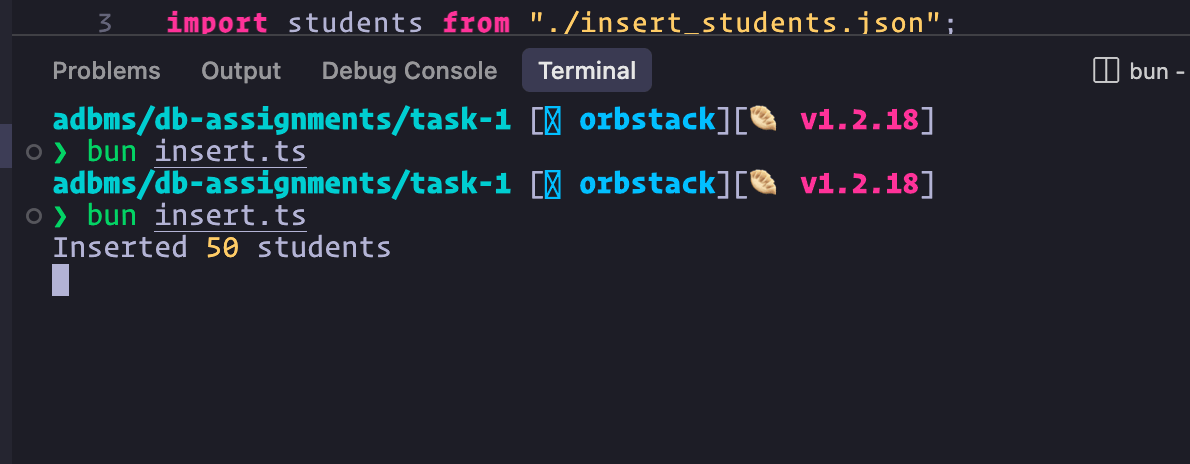
\includegraphics[width=0.8\textwidth]{batch-upsert.png}
\caption{Bulk insert operation output.}
\label{fig:batch-upsert}
\end{figure}

\begin{figure}[H]
\centering
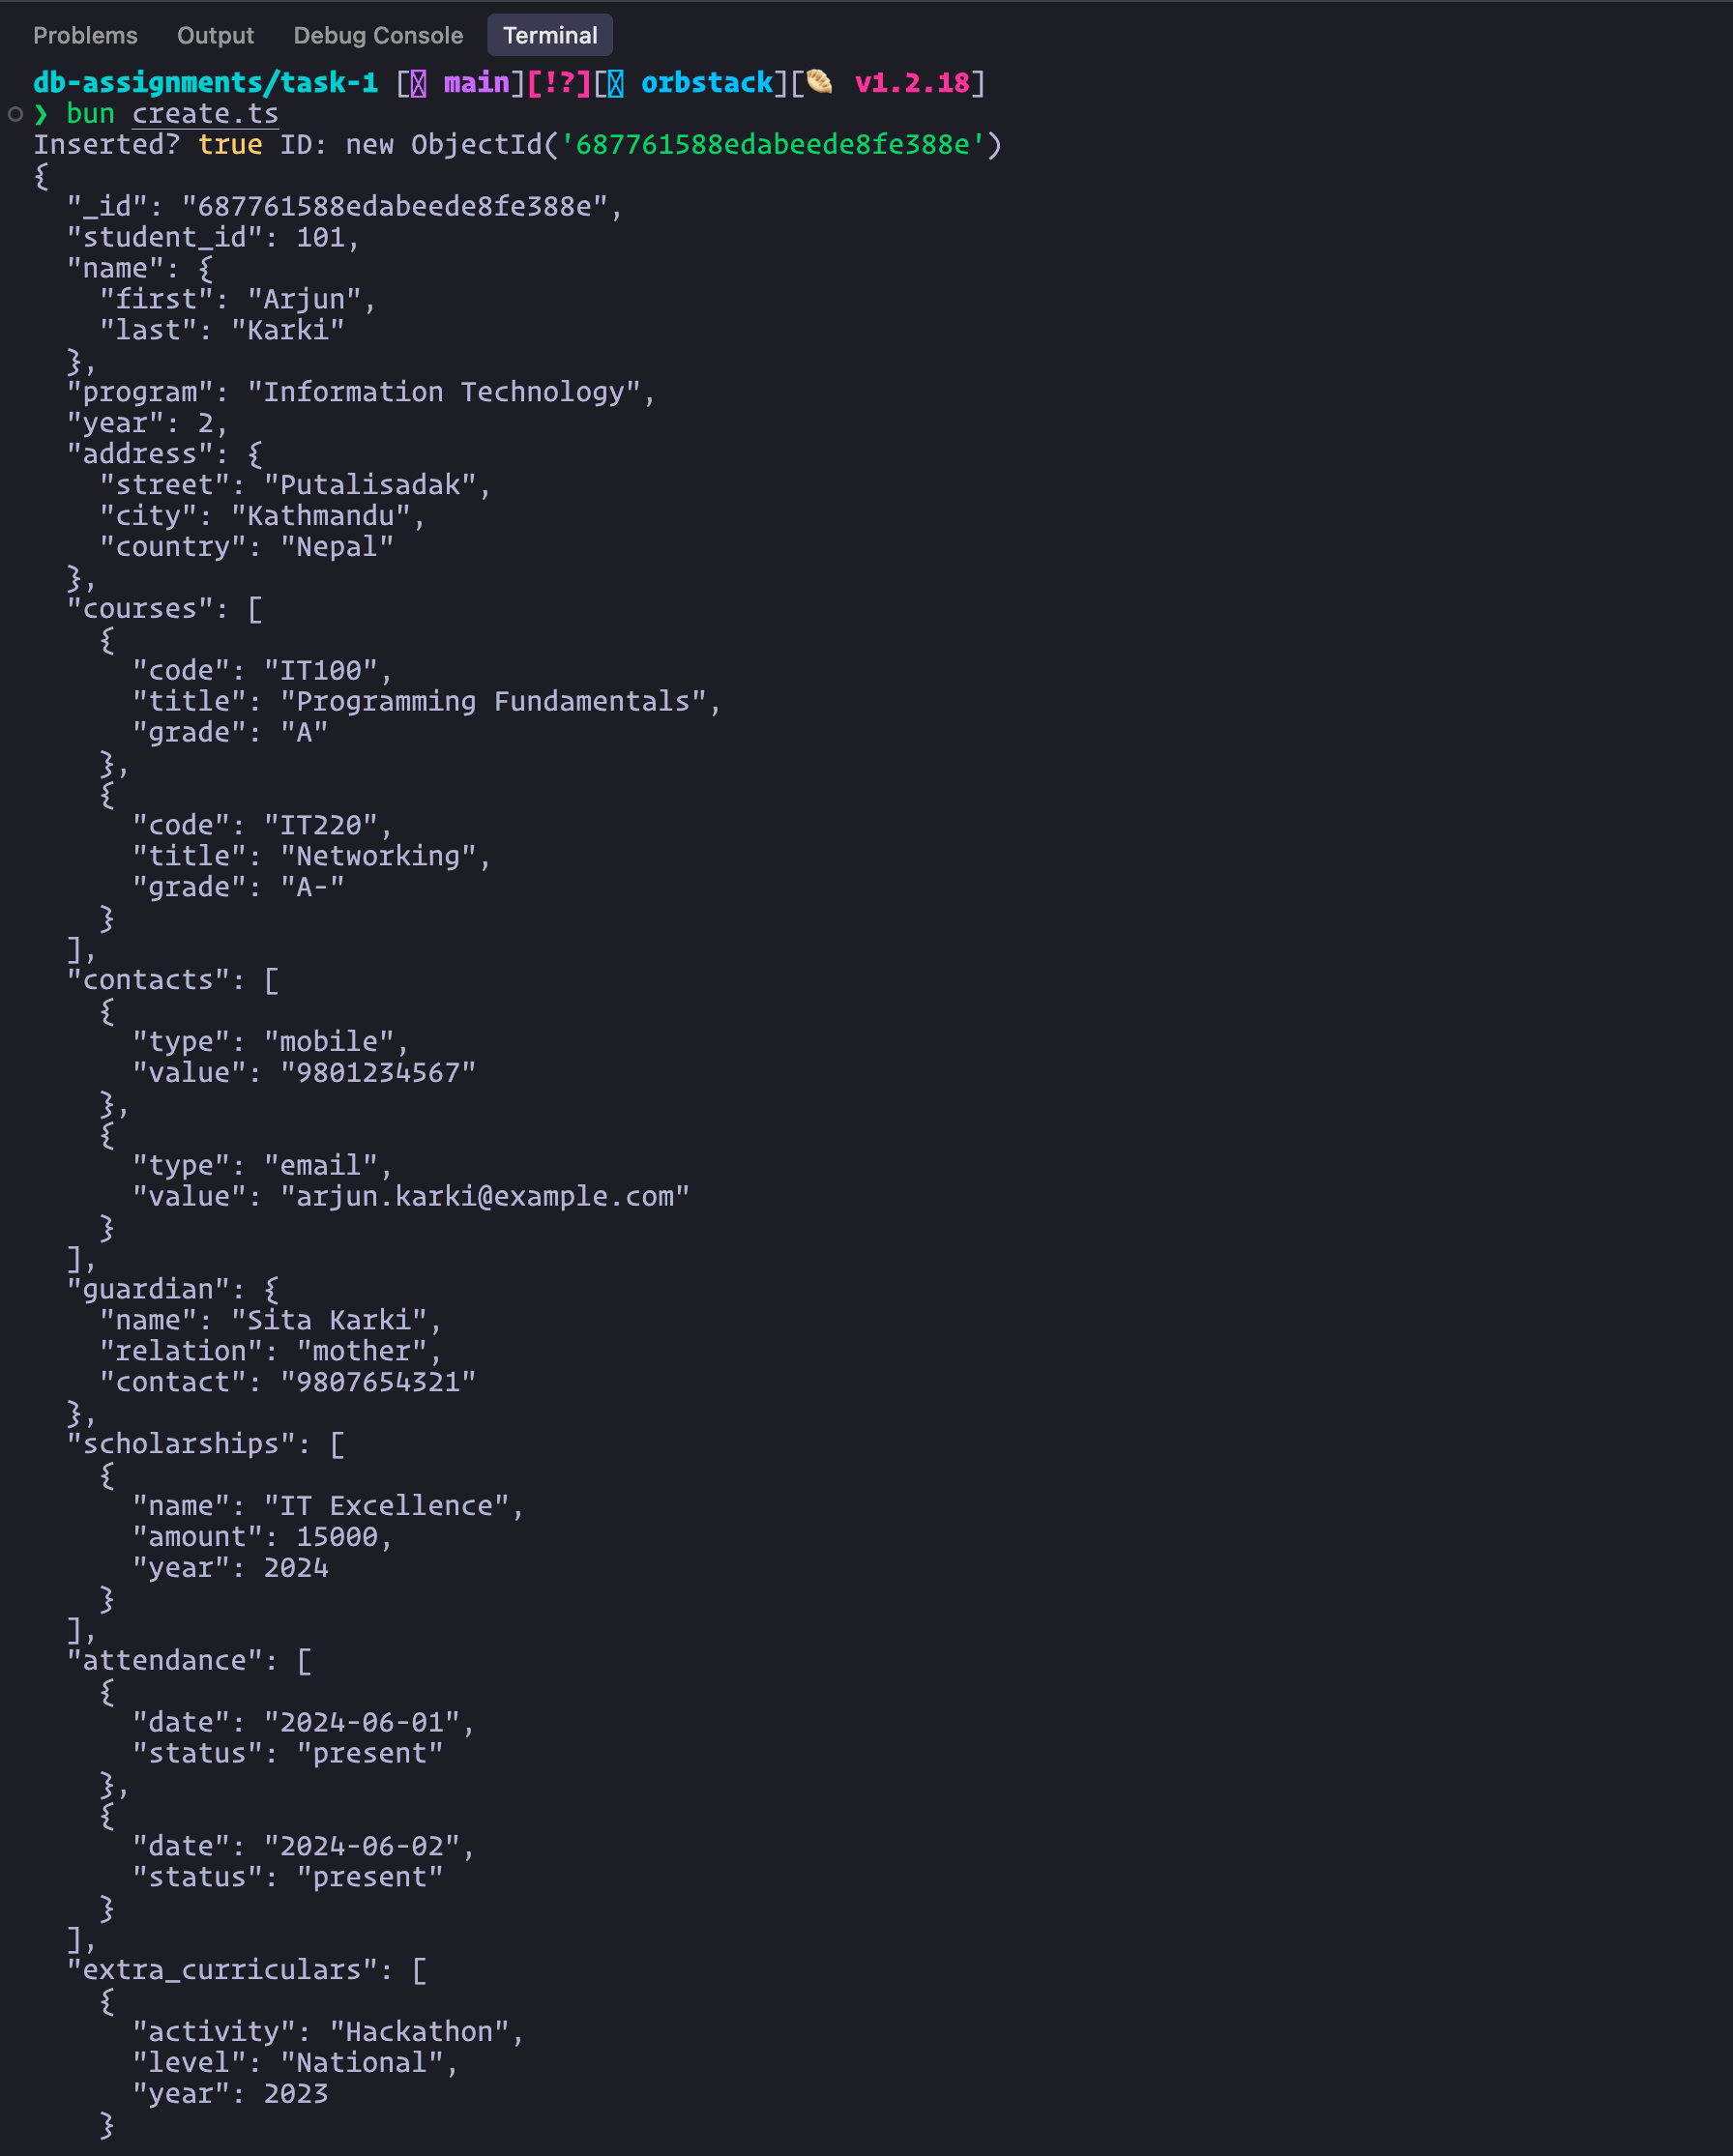
\includegraphics[width=0.8\textwidth]{create-operation-mongo.png}
\caption{Single insert operation output.}
\label{fig:create-operation-mongo}
\end{figure}

\begin{figure}[H]
\centering
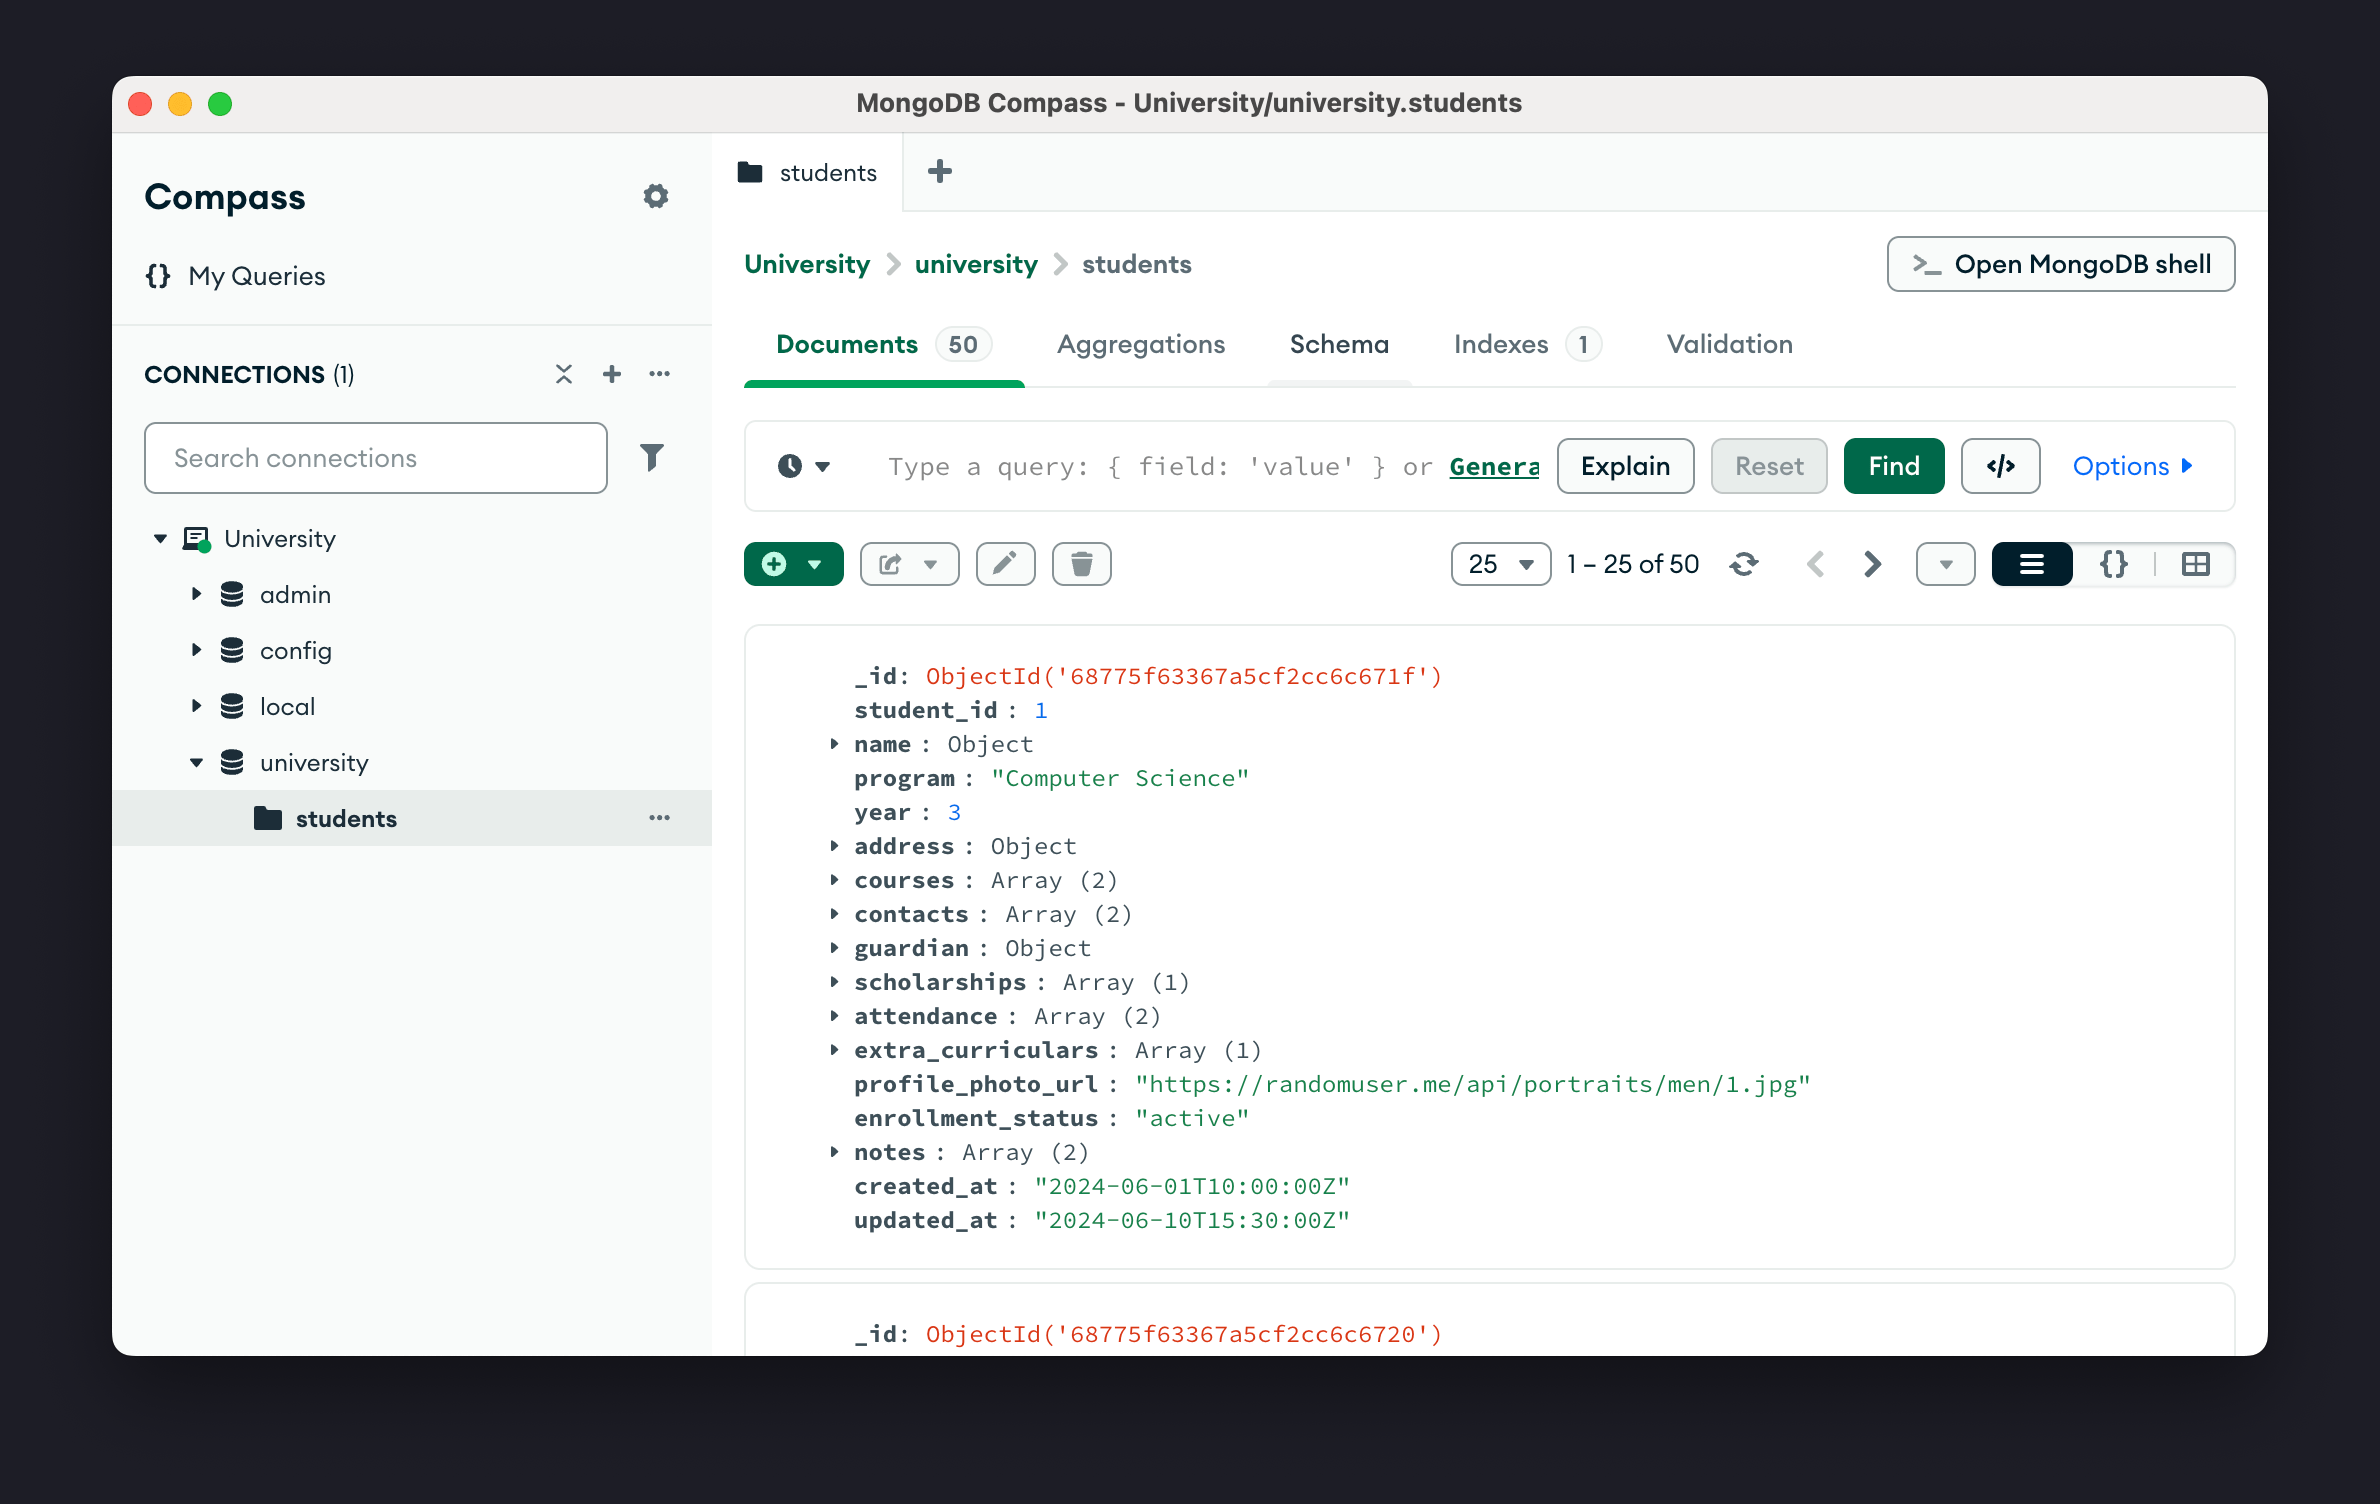
\includegraphics[width=0.8\textwidth]{collection-in-mongodb-compas.png}
\caption{Students collection in MongoDB Compass.}
\label{fig:collection-in-mongodb-compas}
\end{figure}

\begin{figure}[H]
\centering
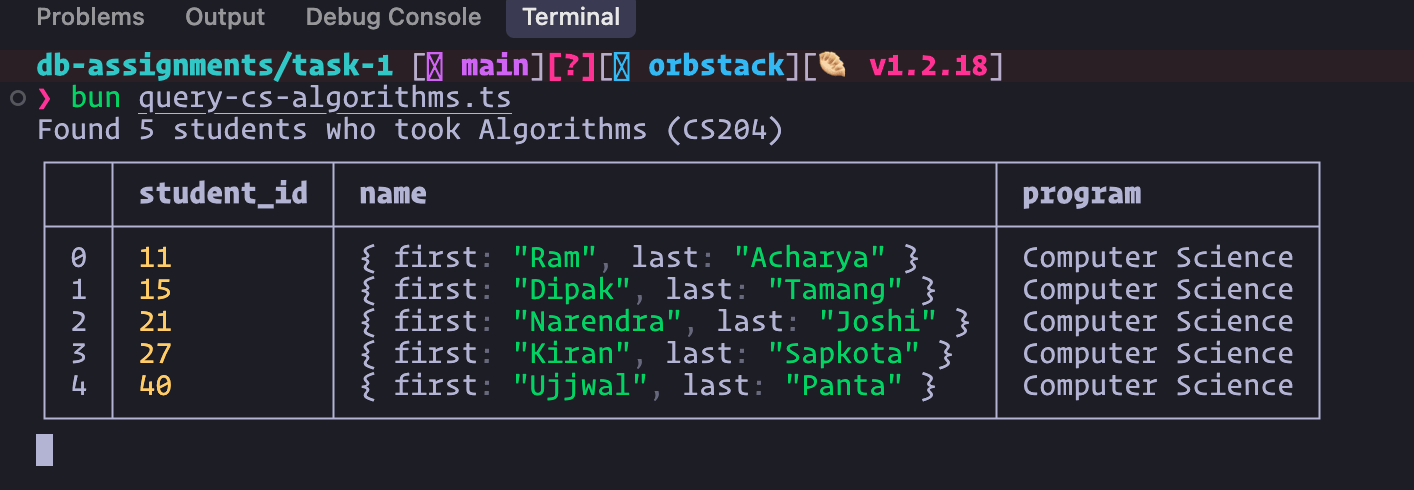
\includegraphics[width=0.8\textwidth]{all-cs-algorithms-204.png}
\caption{CS students who took Algorithms (CS204).}
\label{fig:all-cs-algorithms-204}
\end{figure}

\begin{figure}[H]
\centering
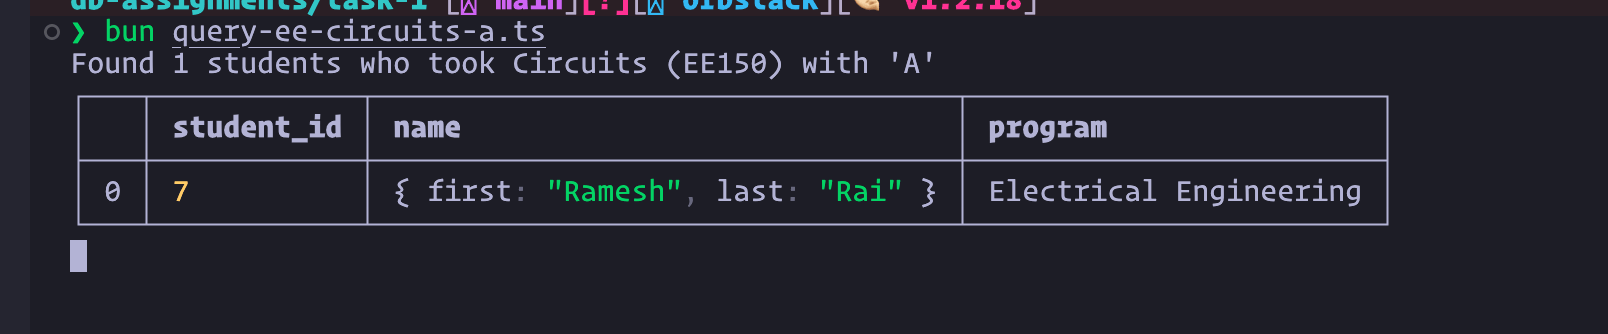
\includegraphics[width=0.8\textwidth]{all-ee-with-A-grade.png}
\caption{EE students with 'A' in Circuits (EE150).}
\label{fig:all-ee-with-A-grade}
\end{figure}

\begin{figure}[H]
\centering
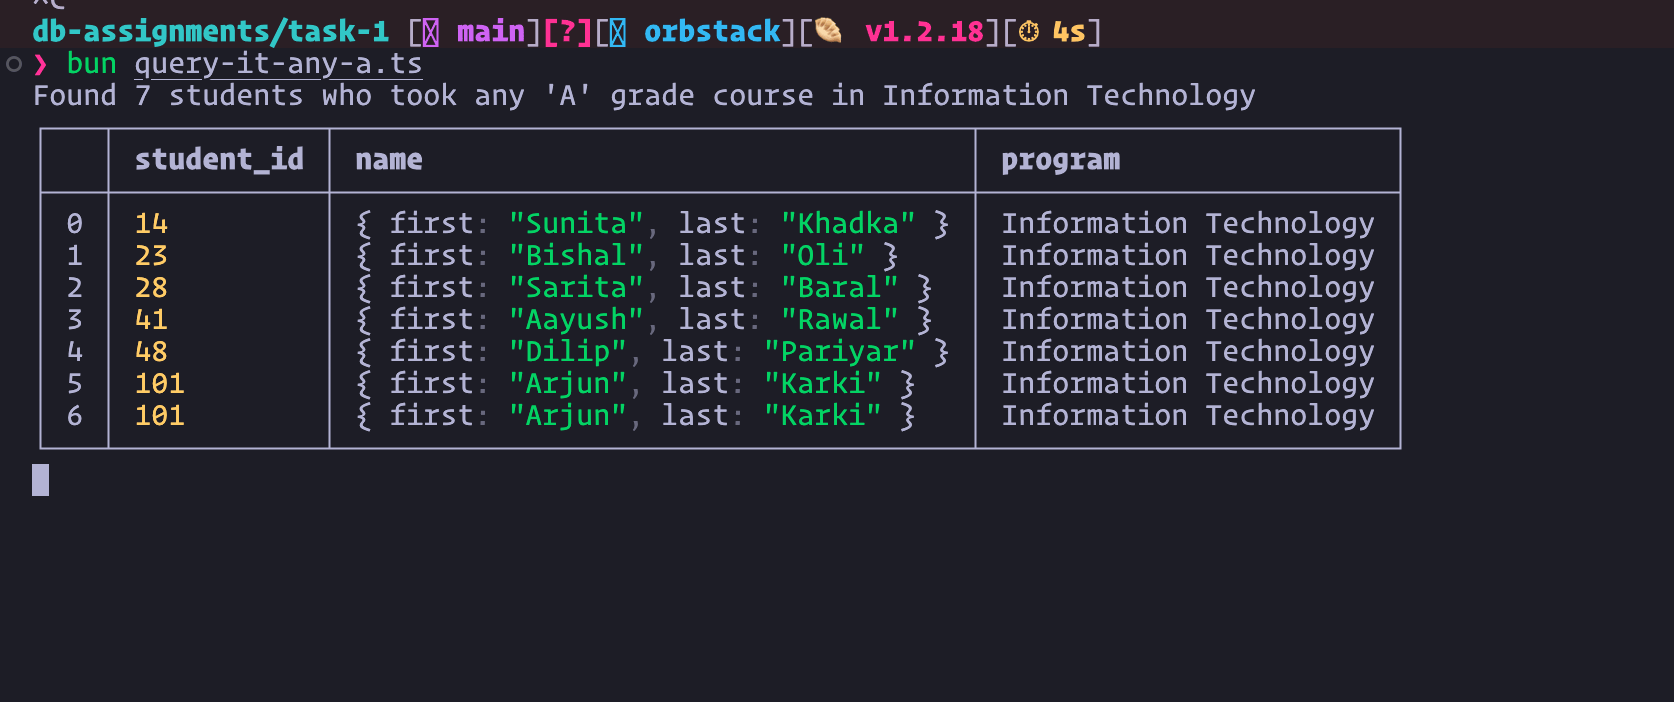
\includegraphics[width=0.8\textwidth]{all-it-with-a-grade.png}
\caption{IT students with any 'A' grade.}
\label{fig:all-it-with-a-grade}
\end{figure}

\begin{figure}[H]
\centering
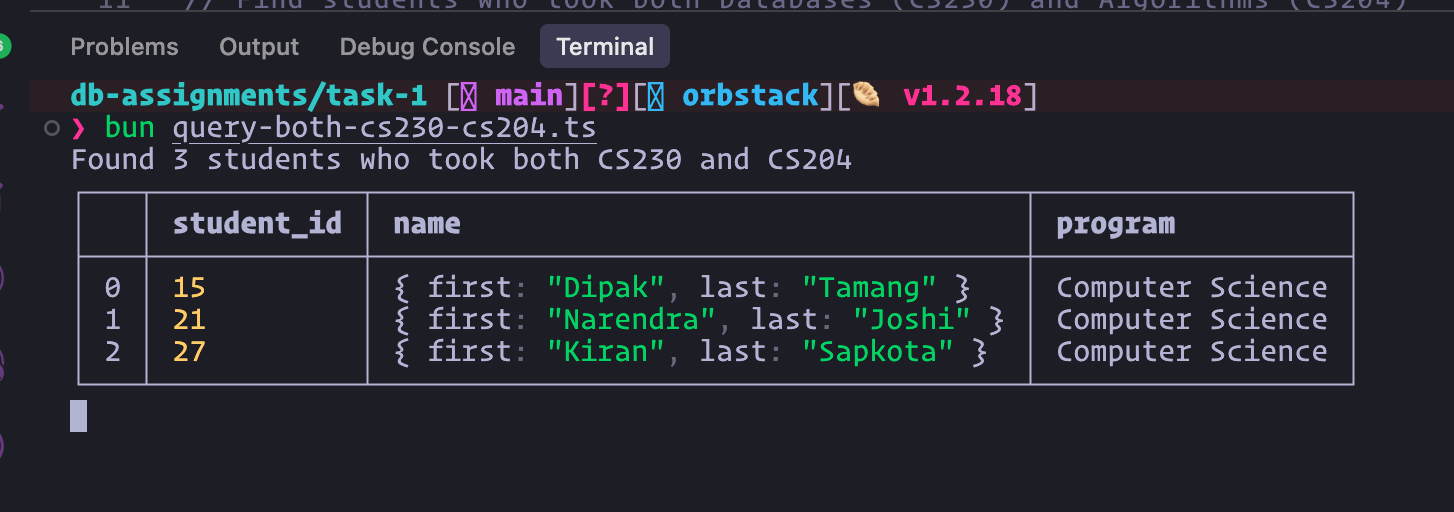
\includegraphics[width=0.8\textwidth]{both-cs230-cs204.png}
\caption{Students who took both CS230 and CS204.}
\label{fig:both-cs230-cs204}
\end{figure}

\begin{figure}[H]
\centering
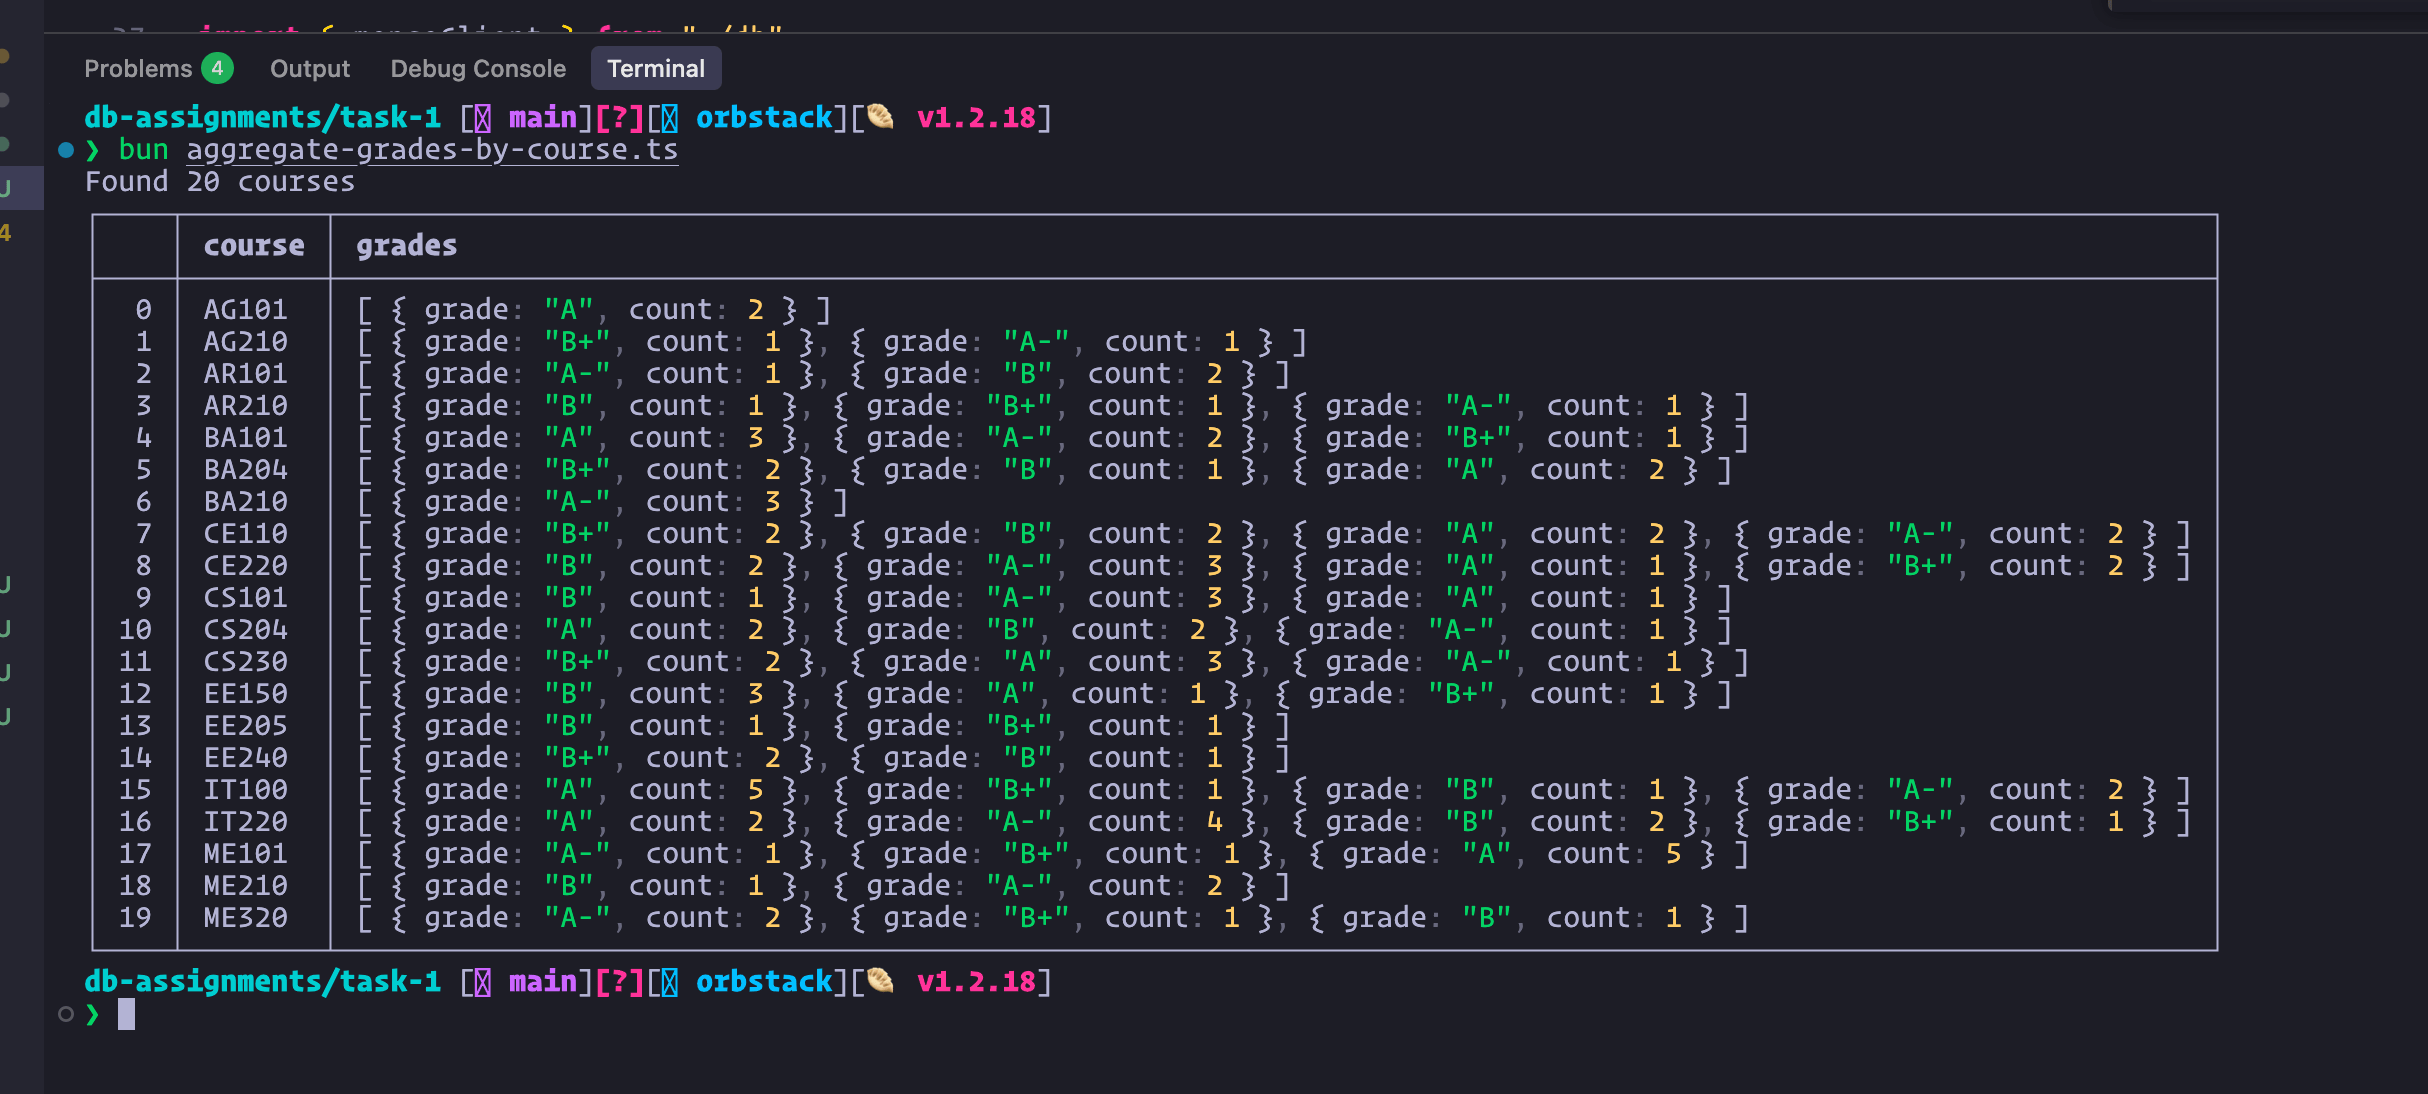
\includegraphics[width=0.8\textwidth]{aggregate-grades-course-code.png}
\caption{Aggregated grades by course.}
\label{fig:aggregate-grades-course-code}
\end{figure}

\begin{figure}[H]
\centering
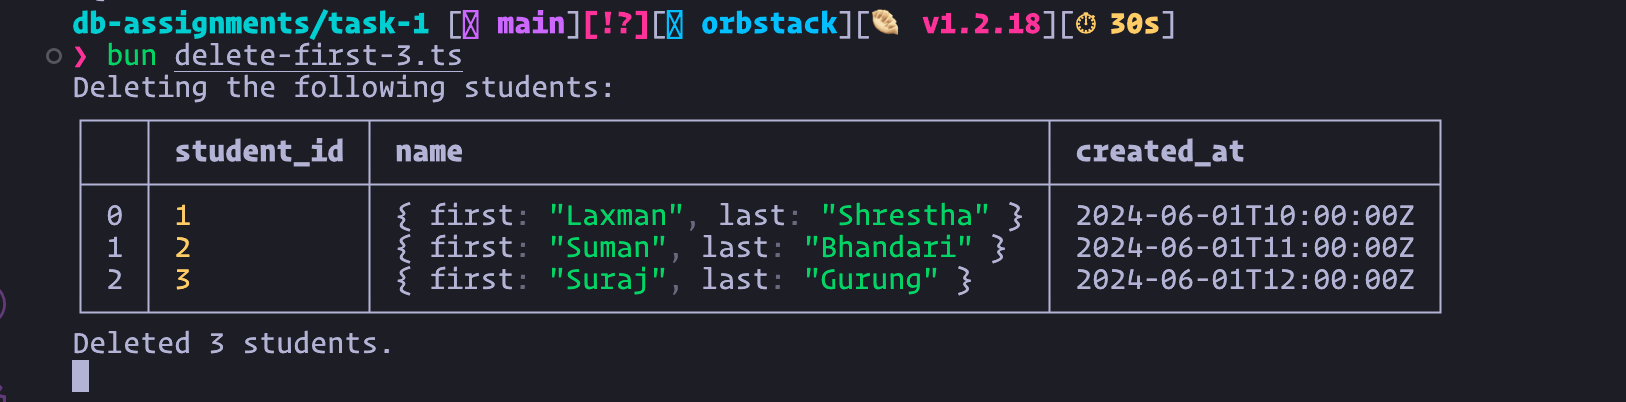
\includegraphics[width=0.8\textwidth]{delete-first-3.png}
\caption{Delete operation output.}
\label{fig:delete-first-3}
\end{figure}

\begin{figure}[H]
  \centering
  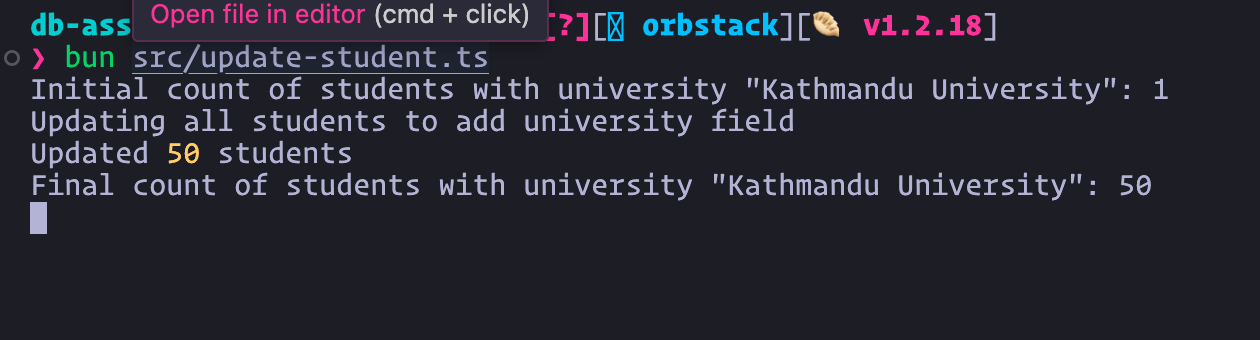
\includegraphics[width=0.8\textwidth]{update-all-university-kathmandu-university.png}
  \caption{Update operation adding university field to all students.}
  \label{fig:update-university}
\end{figure}

\begin{figure}[H]
  \centering
  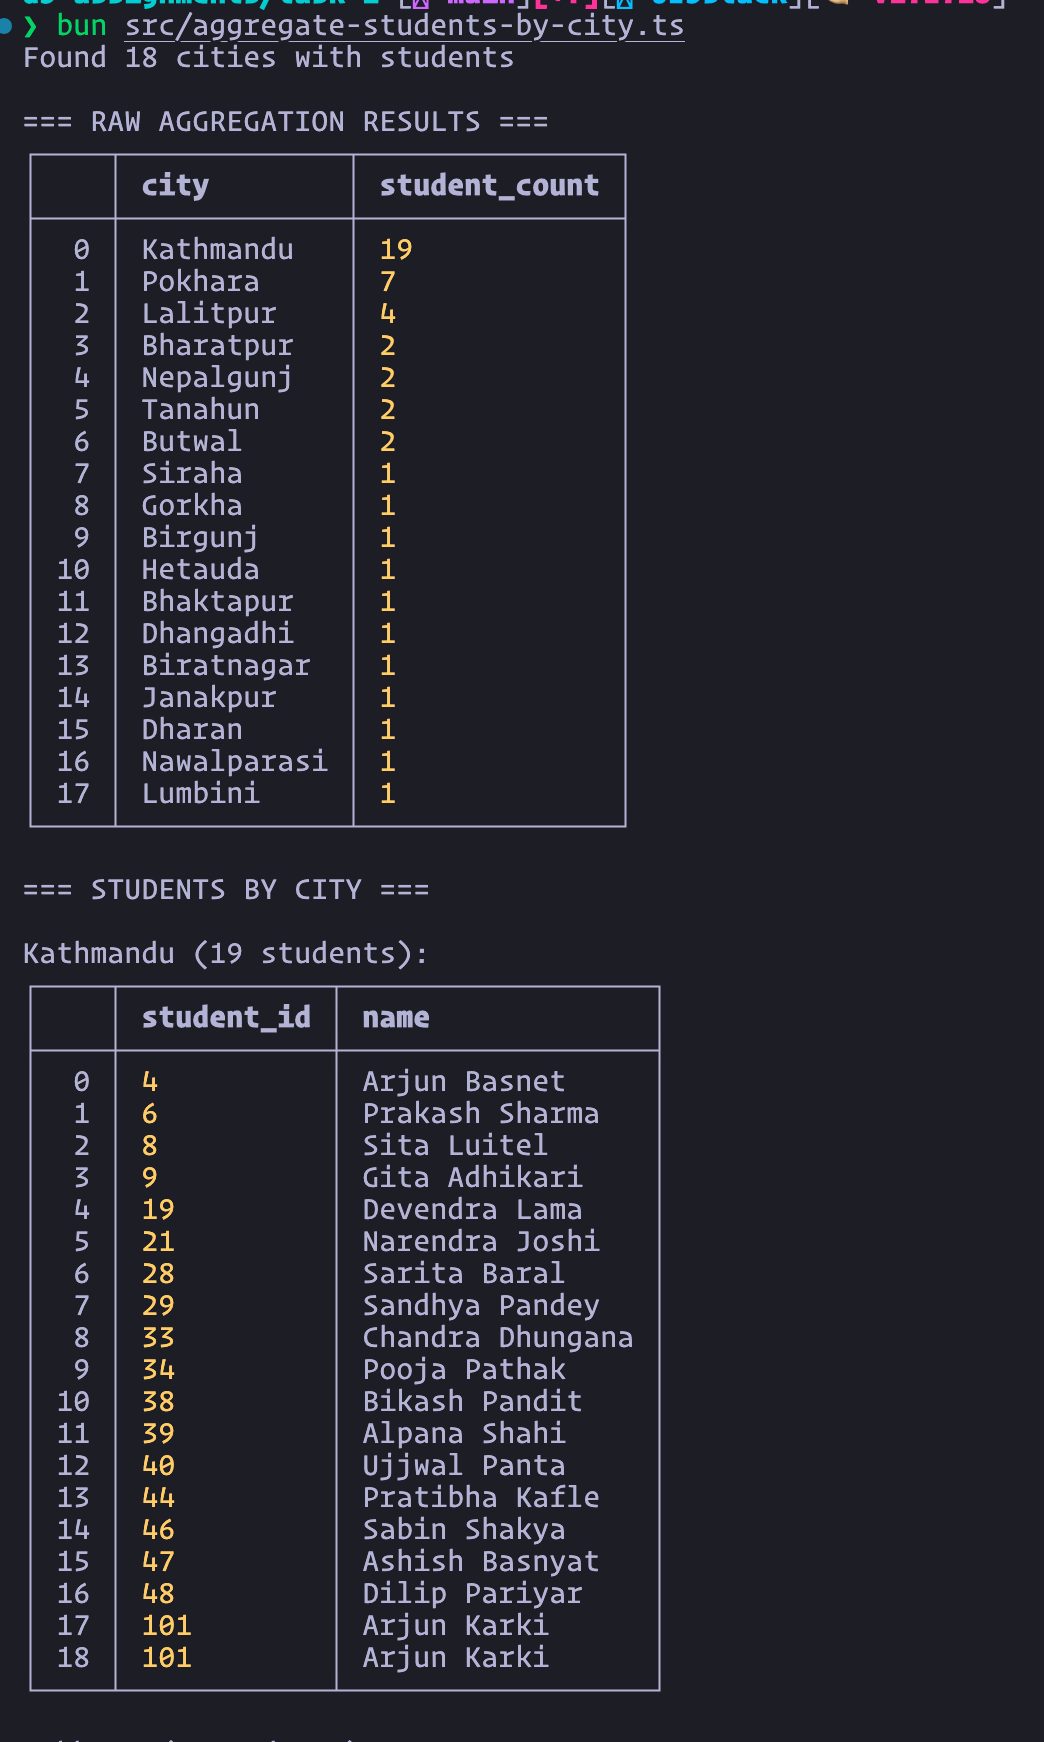
\includegraphics[width=0.8\textwidth]{aggregate-students-by-city.png}
  \caption{Students aggregated and counted by city.}
  \label{fig:aggregate-students-city}
\end{figure}

\begin{figure}[H]
\centering
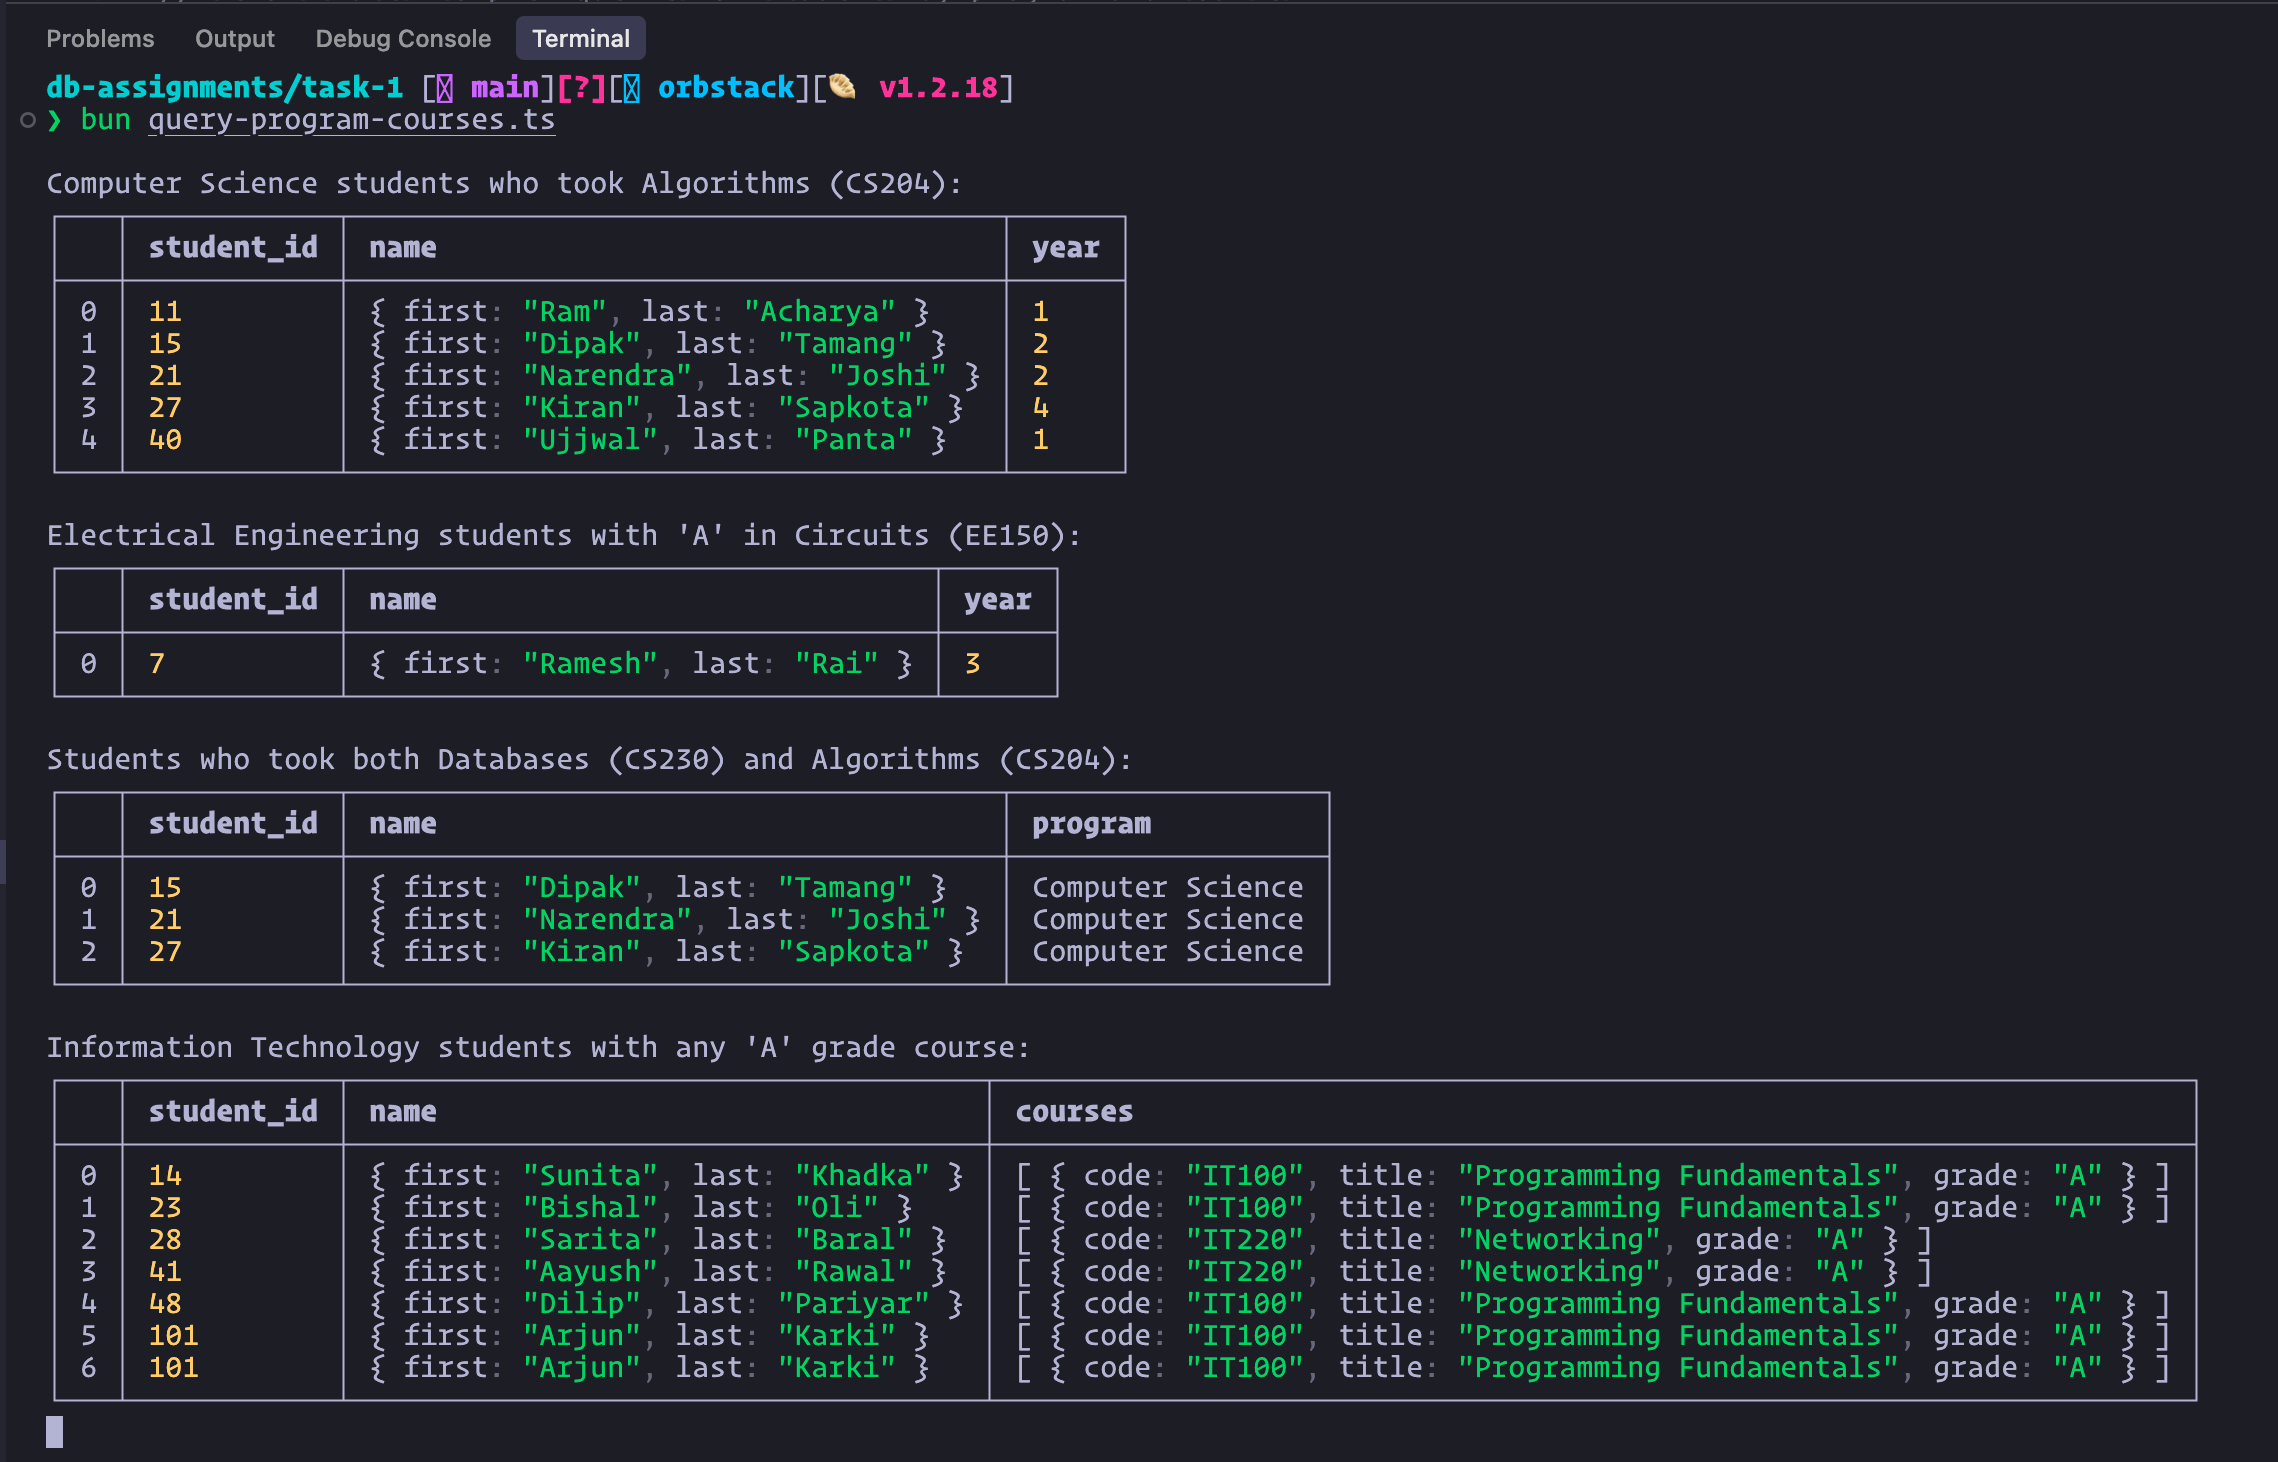
\includegraphics[width=0.8\textwidth]{program-courses.png}
\caption{Student programs and courses overview.}
\label{fig:program-courses}
\end{figure}

\section{Cassandra Wide-Column Database Screenshots}

The following screenshots document the implementation and operation of the Apache Cassandra-based attendance system, demonstrating schema creation, data insertion, and various query operations.

\begin{figure}[H]
  \centering
  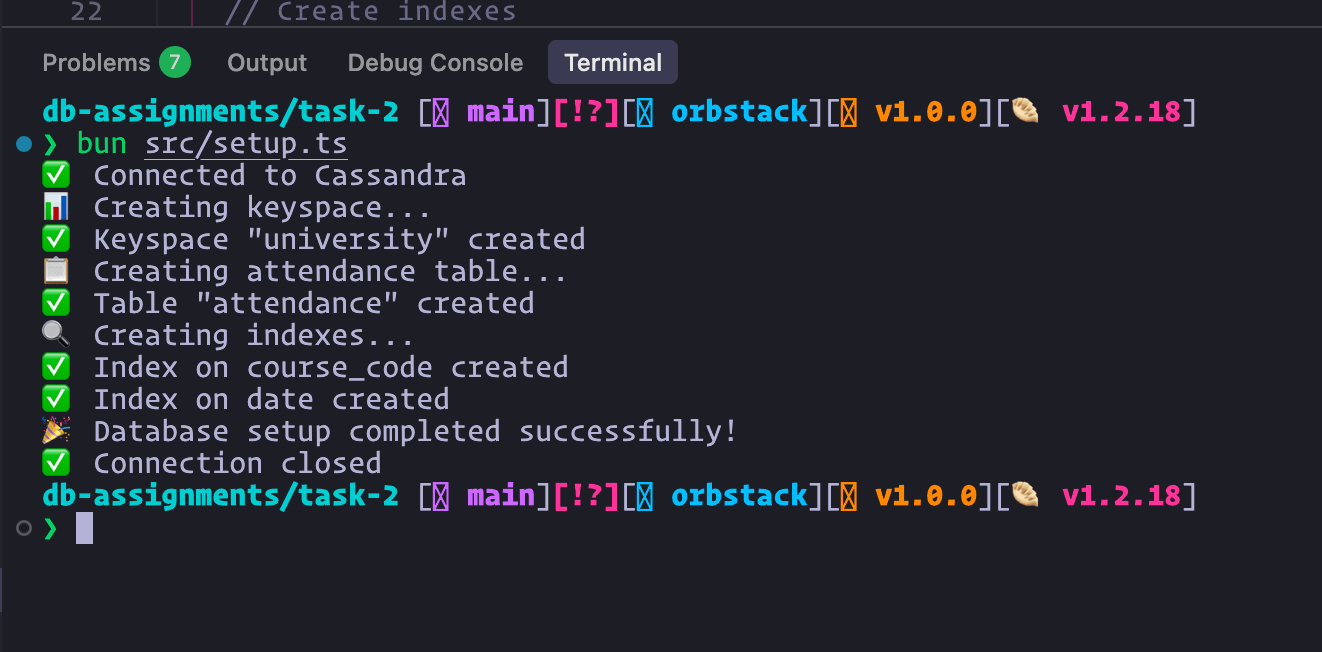
\includegraphics[width=0.8\textwidth]{task-2/screenshots/create-database-and-tables.png}
  \caption{Database Schema Creation: Terminal output showing the successful creation of the \texttt{university} keyspace, \texttt{attendance} table with composite primary key (student\_id, course\_code, date), and secondary indexes for course\_code and date fields. This demonstrates the initial setup phase of the Cassandra database.}
  \label{fig:task2-create-database}
\end{figure}

\begin{figure}[H]
  \centering
  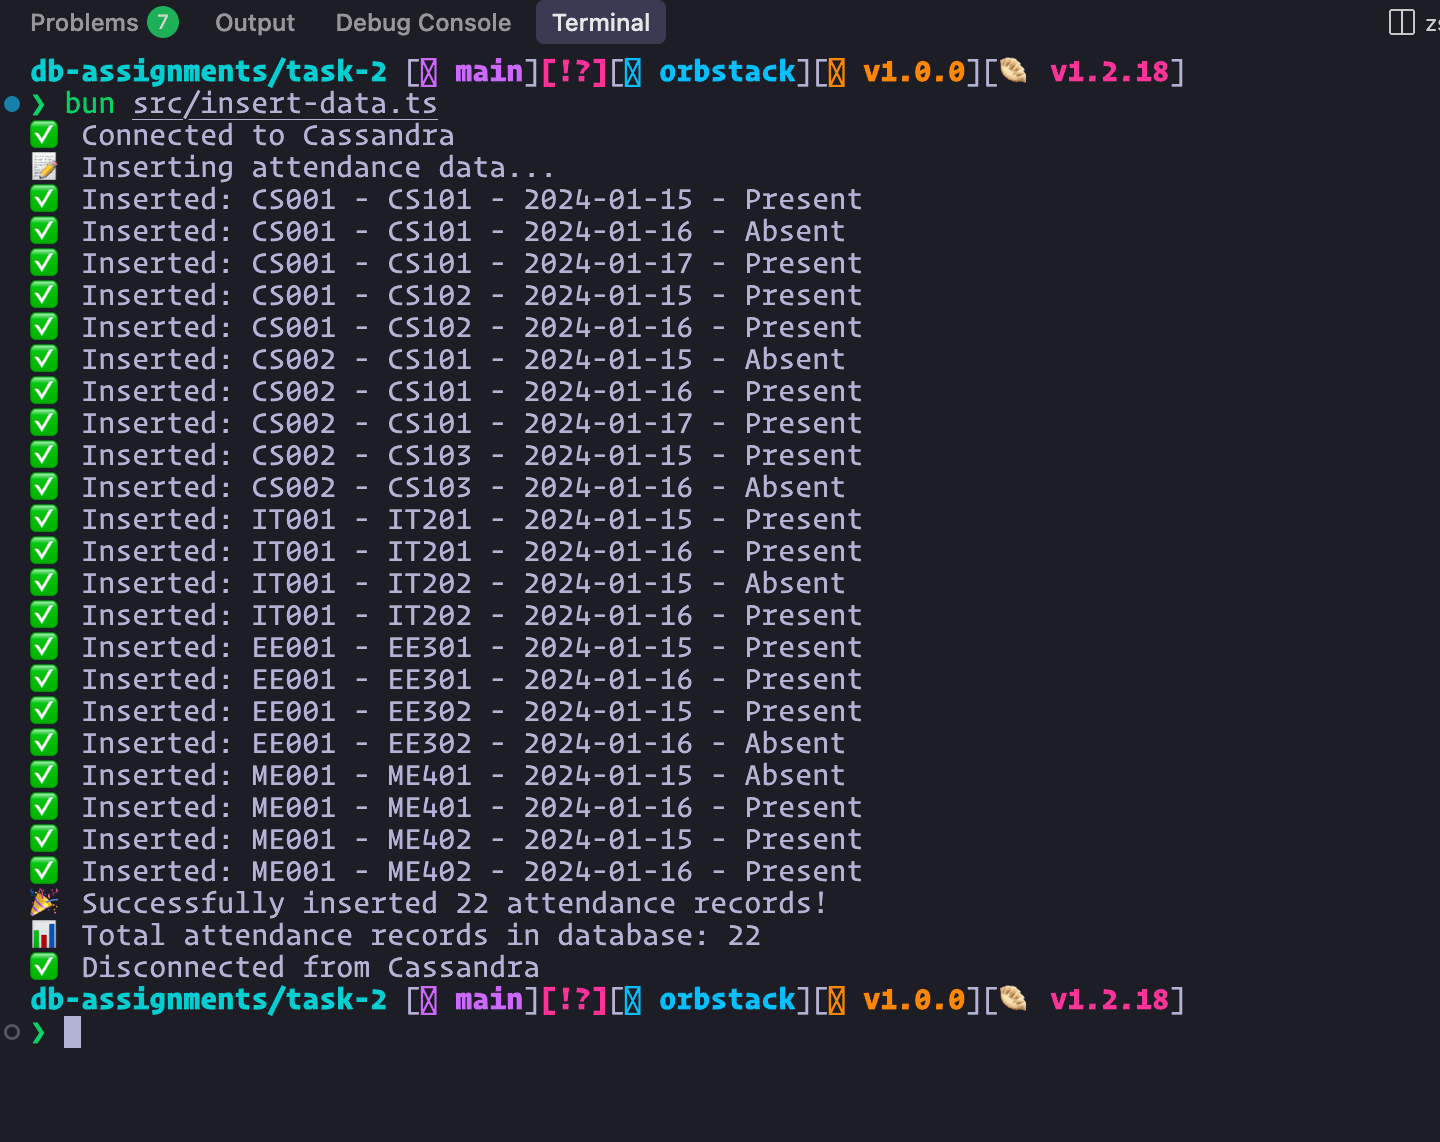
\includegraphics[width=0.8\textwidth]{task-2/screenshots/insert-data.png}
  \caption{Bulk Data Insertion Process: Console output displaying the sequential insertion of 22 attendance records across 5 students from different departments (CS, IT, EE, ME). Each record shows the student ID, course code, date, and attendance status, demonstrating the data loading phase with TypeScript/Node.js driver.}
  \label{fig:task2-insert-data}
\end{figure}

\begin{figure}[H]
  \centering
  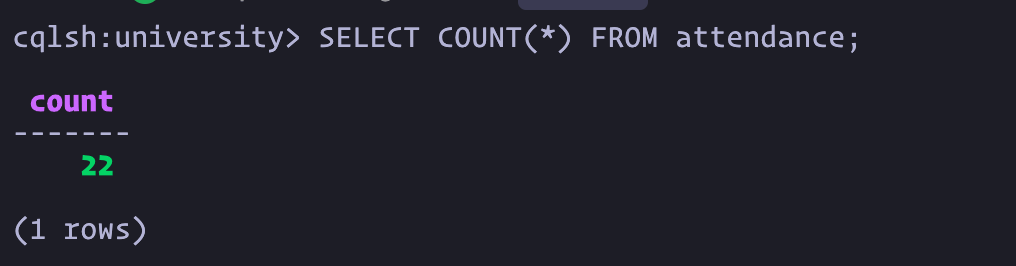
\includegraphics[width=0.8\textwidth]{task-2/screenshots/count_query.png}
  \caption{Record Count Verification: Execution of \texttt{SELECT COUNT(*) FROM attendance} query showing the total number of records (22) successfully inserted into the database. This validates the data insertion process and demonstrates basic aggregation functionality.}
  \label{fig:task2-count-query}
\end{figure}

\begin{figure}[H]
  \centering
  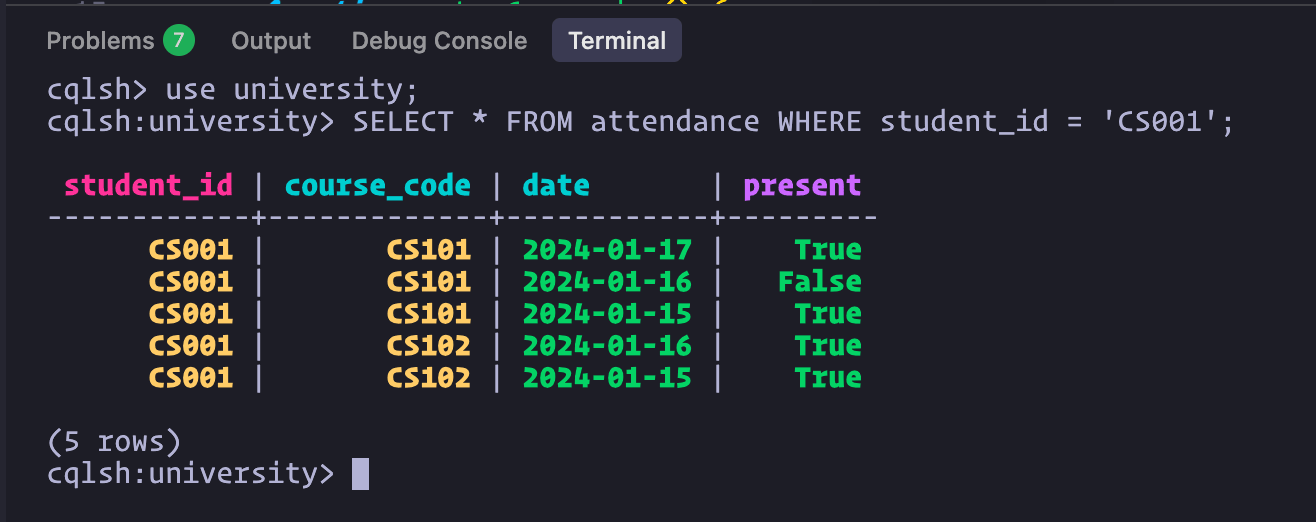
\includegraphics[width=0.8\textwidth]{task-2/screenshots/select-where_student_id.png}
  \caption{Student-Specific Query Results: Output of \texttt{SELECT * FROM attendance WHERE student\_id = 'CS001'} showing all attendance records for student CS001 across multiple courses (CS101, CS102) and dates. This demonstrates efficient partition key-based querying with optimal performance.}
  \label{fig:task2-select-student}
\end{figure}

\begin{figure}[H]
  \centering
  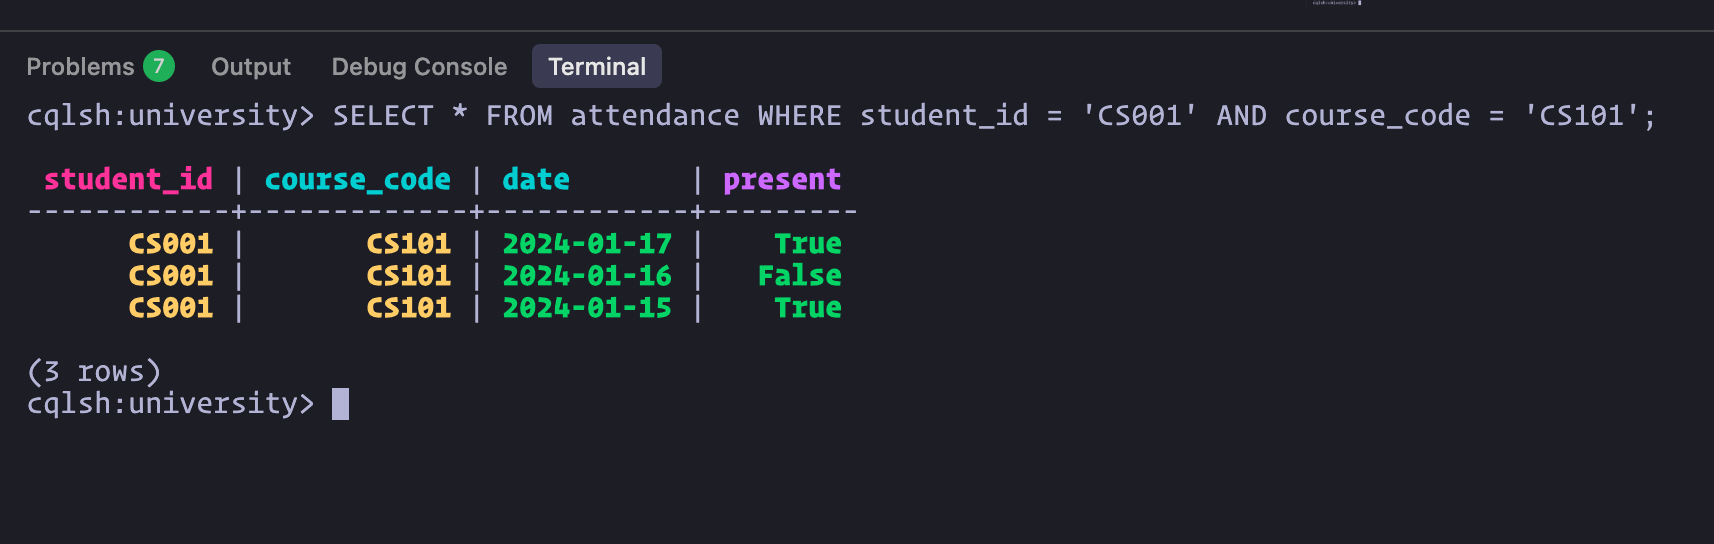
\includegraphics[width=0.8\textwidth]{task-2/screenshots/select-where_student_id_and_course_code.png}
  \caption{Student and Course-Specific Query: Results from \texttt{SELECT * FROM attendance WHERE student\_id = 'CS001' AND course\_code = 'CS101'} displaying attendance records for a specific student-course combination. This showcases the efficiency of using both partition key (student\_id) and clustering key (course\_code).}
  \label{fig:task2-select-student-course}
\end{figure}

\begin{figure}[H]
  \centering
  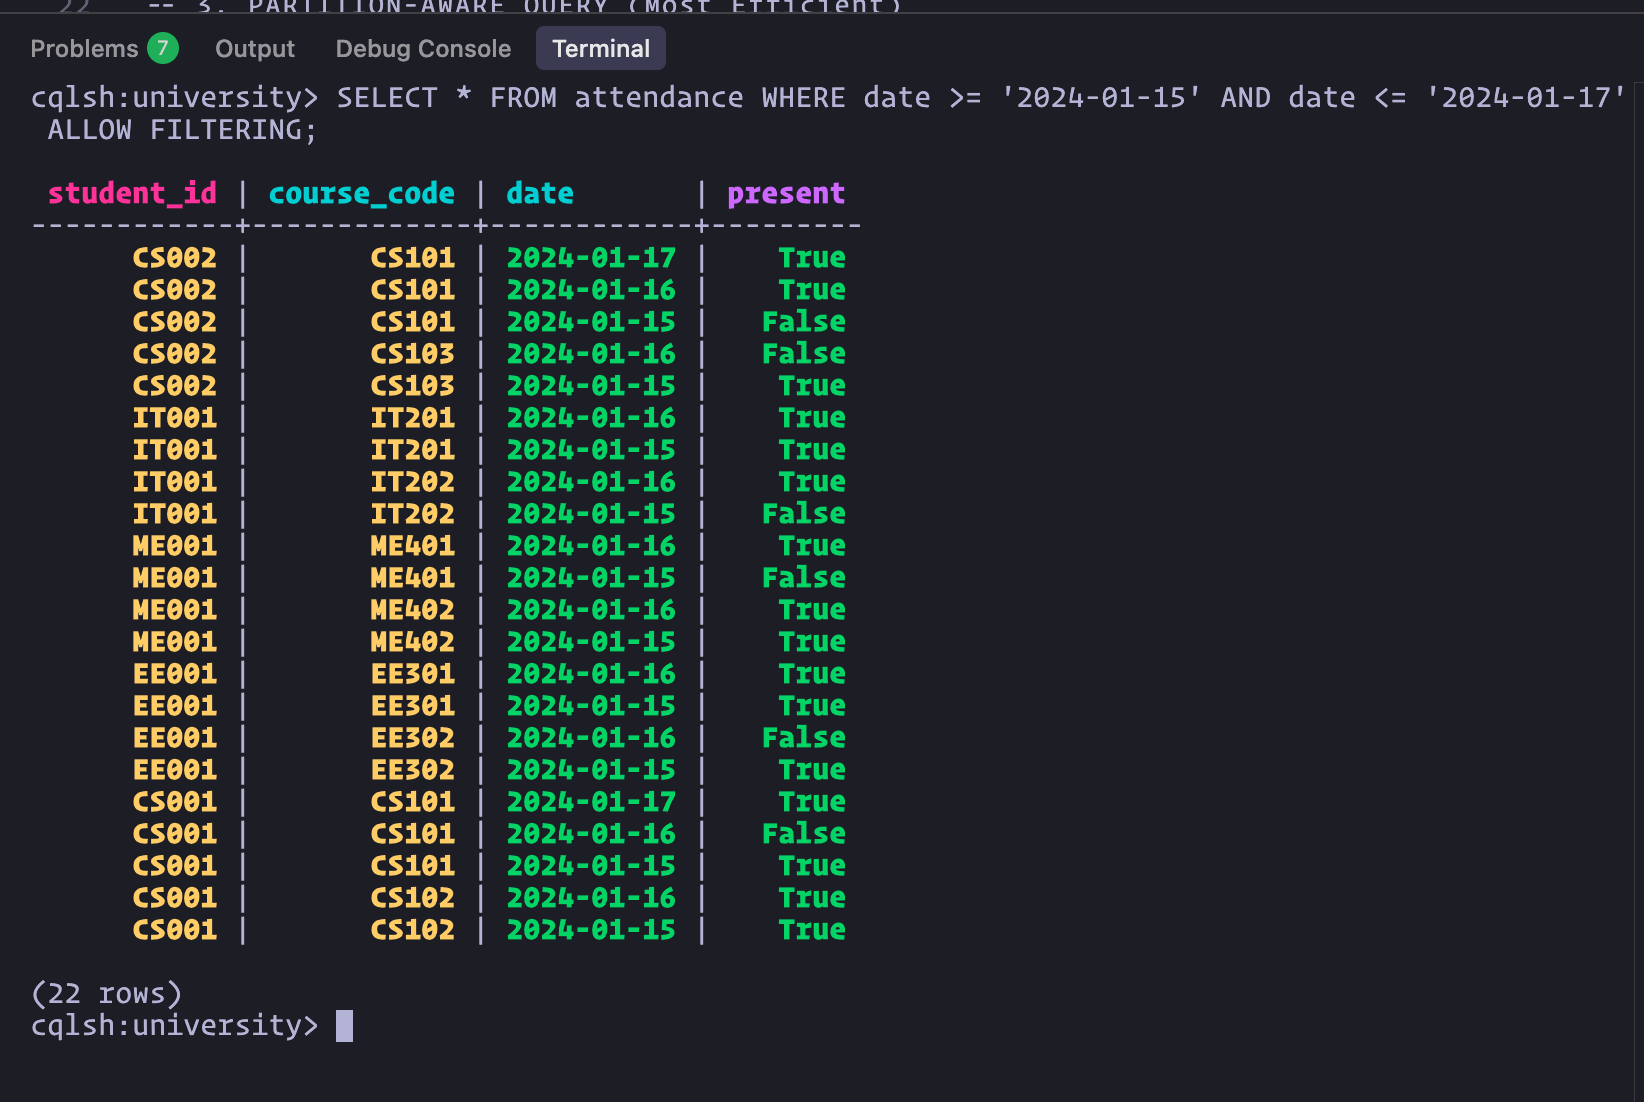
\includegraphics[width=0.8\textwidth]{task-2/screenshots/date_range_query.png}
  \caption{Date Range Query Implementation: Demonstration of time-based queries using secondary indexes on the date field. This shows how the system can efficiently retrieve attendance records within specific time periods, essential for generating attendance reports by date ranges.}
  \label{fig:task2-date-range}
\end{figure}

\begin{figure}[H]
  \centering
  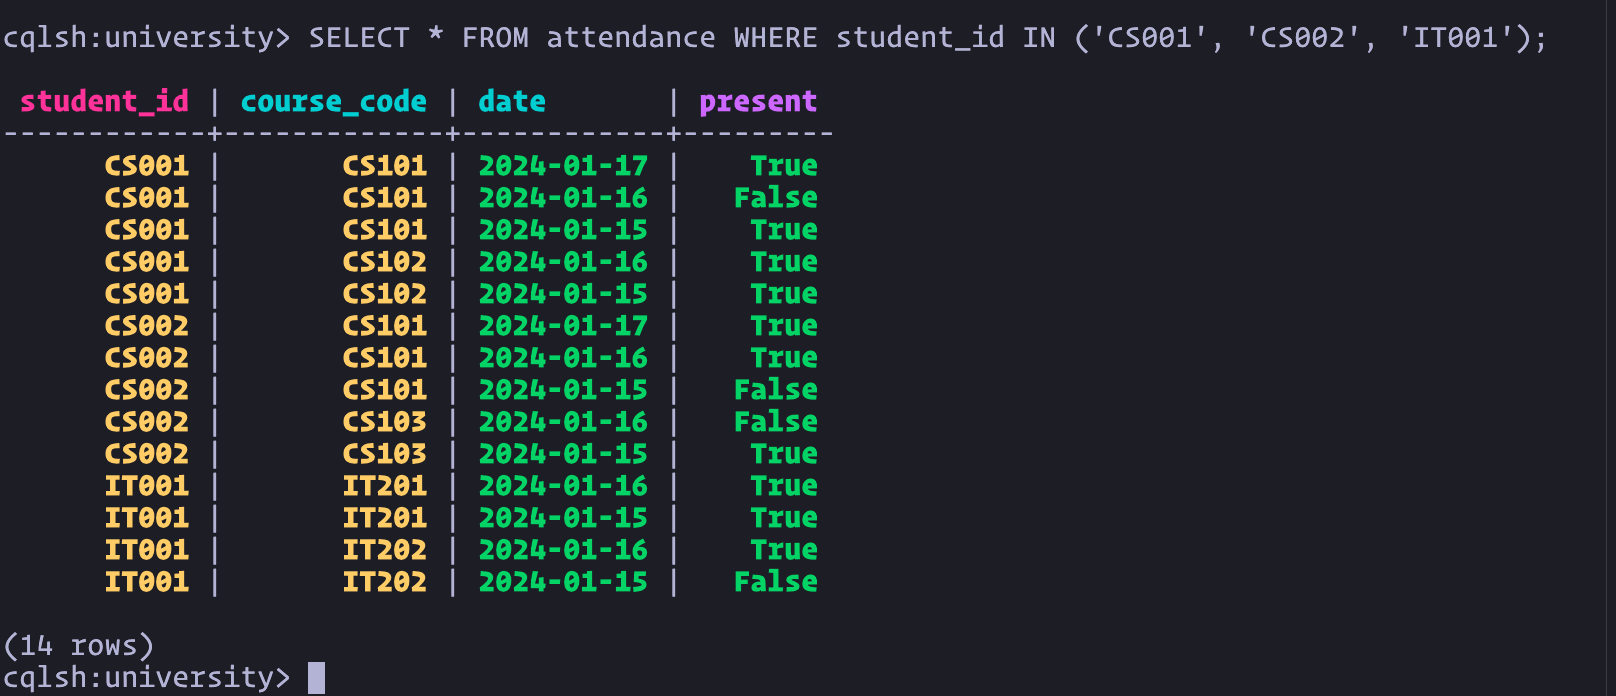
\includegraphics[width=0.8\textwidth]{task-2/screenshots/where_query.png}
  \caption{Advanced WHERE Clause Operations: Complex query examples demonstrating various filtering conditions and query patterns supported by the Cassandra schema. This includes compound conditions and the use of secondary indexes for flexible data retrieval.}
  \label{fig:task2-where-query}
\end{figure}

\begin{figure}[H]
  \centering
  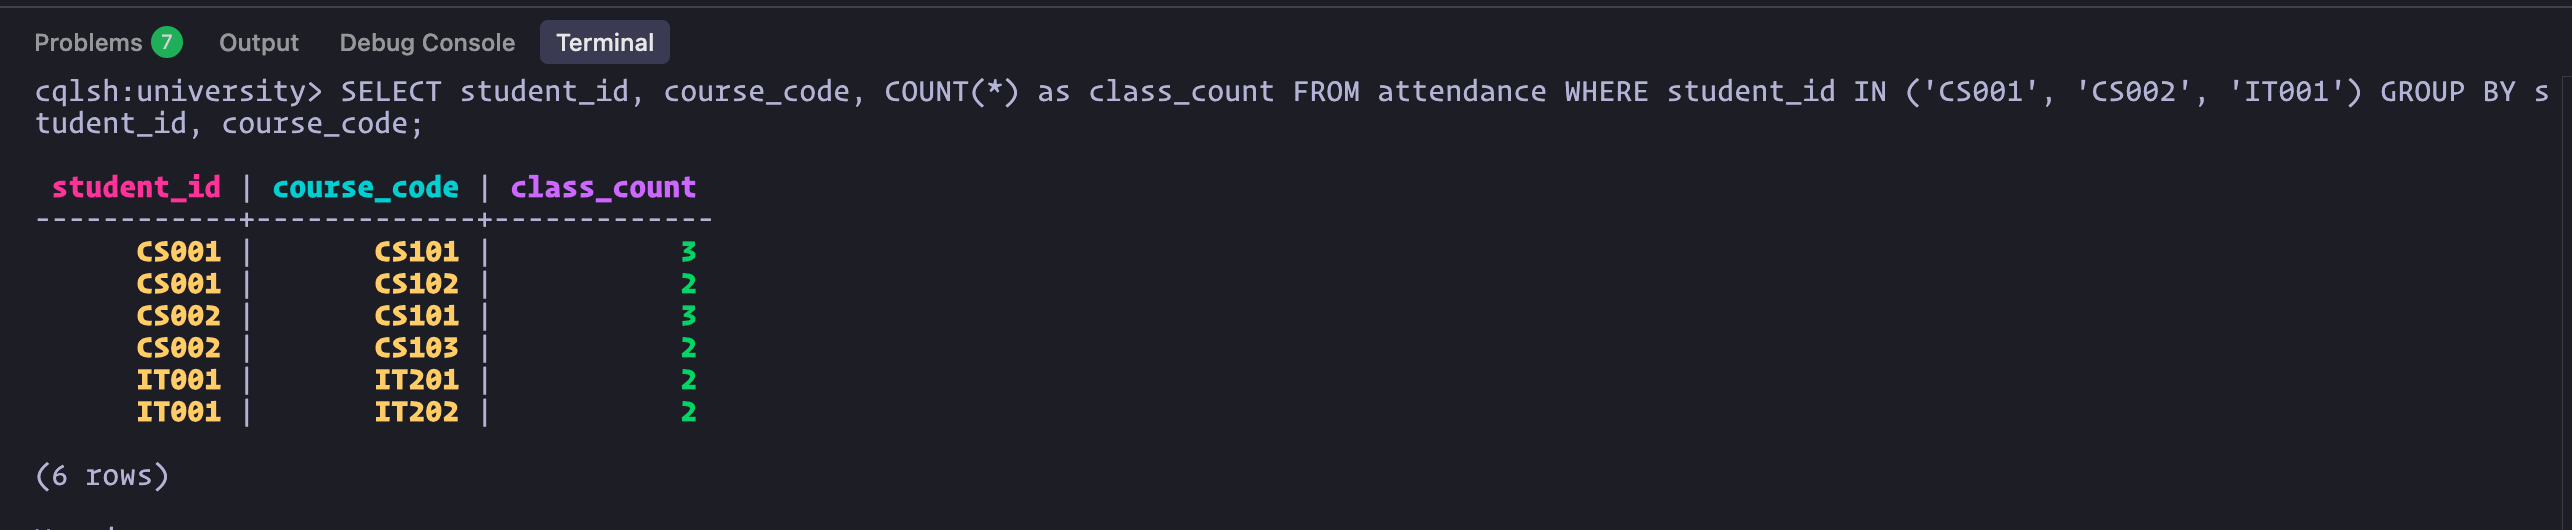
\includegraphics[width=0.8\textwidth]{task-2/screenshots/student-course-group.png}
  \caption{Grouping and Aggregation Analysis: Advanced analytical queries showing student-course relationship analysis and attendance pattern grouping. This demonstrates Cassandra's capability for data aggregation and reporting, useful for generating attendance statistics and academic performance insights.}
  \label{fig:task2-student-course-group}
\end{figure}

\section{Neo4j Graph Database Screenshots}

The following screenshots document the implementation and operation of the Neo4j-based university system. Neo4j Browser was used to execute Cypher queries and visualize the graph structure. Each screenshot demonstrates different aspects of graph database operations, from data setup to complex relationship queries. For detailed query results and explanations, see the Neo4j implementation section.

\subsection*{Database Setup and Graph Creation}

\begin{figure}[H]
  \centering
  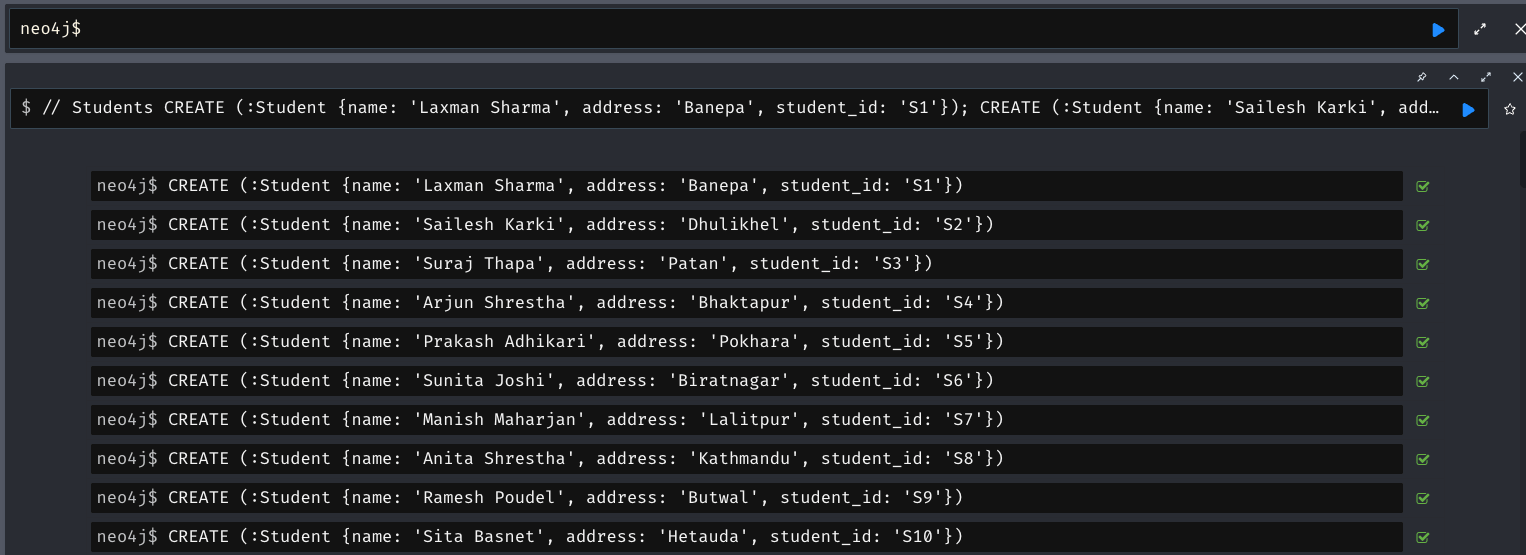
\includegraphics[width=0.8\textwidth]{task-3/screenshots/import-data.png}
  \caption{Data Import Process: Screenshot showing the execution of Cypher commands to create nodes for Students, Professors, and Courses in the Neo4j database. This demonstrates the initial data loading phase where entities are created with their respective properties.}
  \label{fig:task3-import-data}
\end{figure}

\begin{figure}[H]
  \centering
  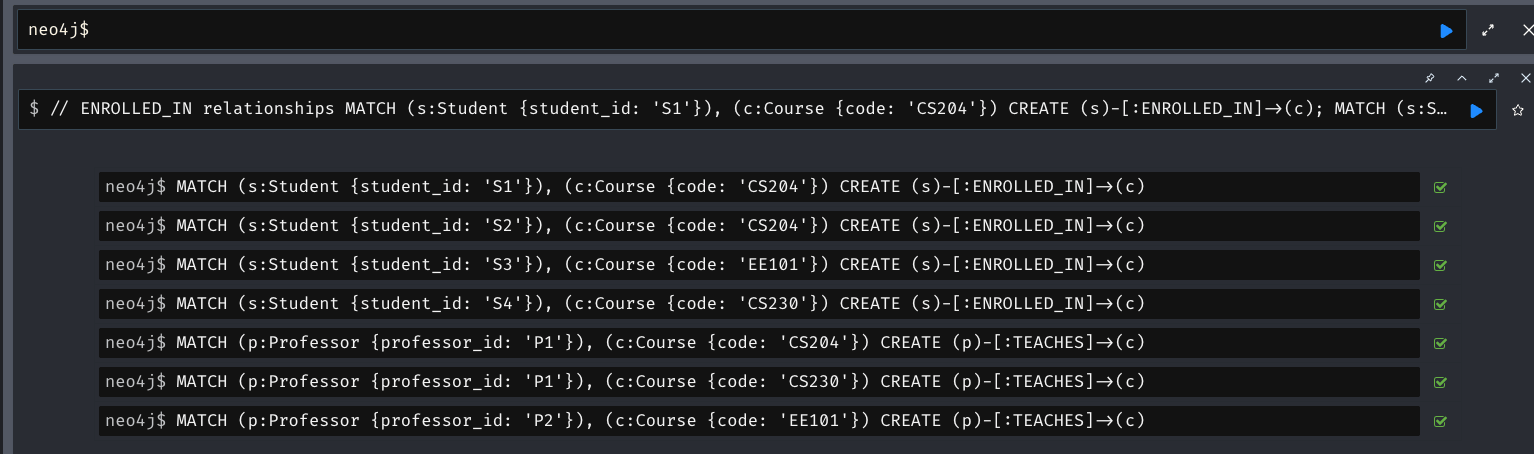
\includegraphics[width=0.8\textwidth]{task-3/screenshots/create-relationships.png}
  \caption{Relationship Creation: Screenshot displaying the creation of ENROLLED\_IN and TEACHES relationships between nodes. This establishes the connections that define how students relate to courses and how professors relate to courses in the graph structure.}
  \label{fig:task3-create-relationships}
\end{figure}

\subsection*{Cypher Query Results}

\begin{figure}[H]
  \centering
  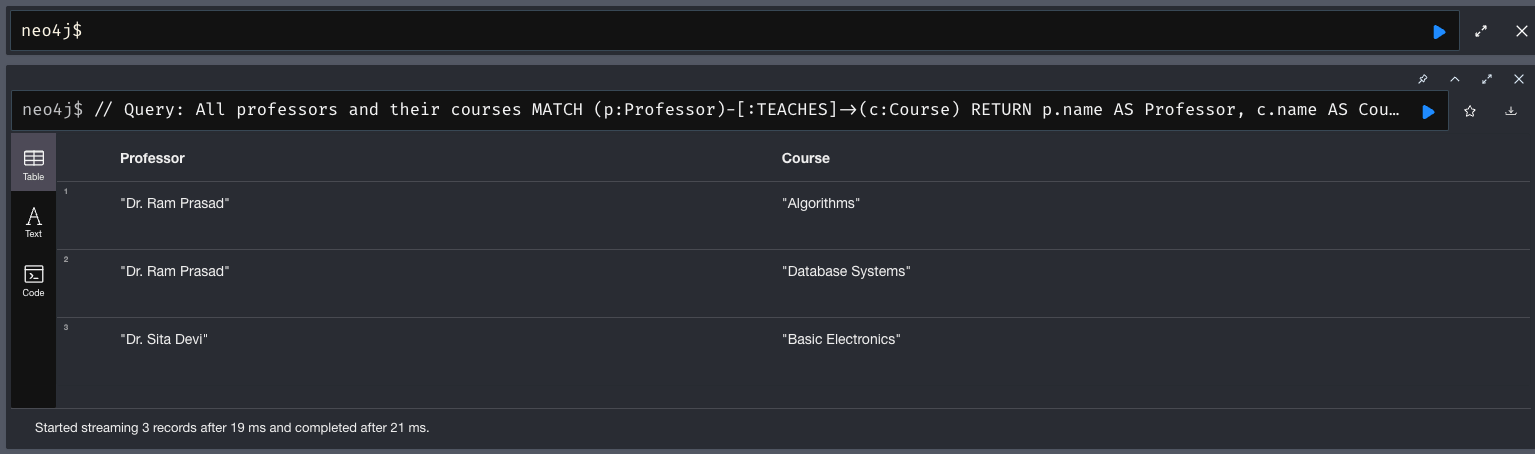
\includegraphics[width=0.8\textwidth]{task-3/screenshots/all-prof-and-their-courses.png}
  \caption{Query Result: All professors and their courses. This screenshot shows the output of a Cypher query that retrieves all professors and the courses they teach, demonstrating basic graph traversal using the TEACHES relationship.}
  \label{fig:task3-all-prof-courses}
\end{figure}

\begin{figure}[H]
  \centering
  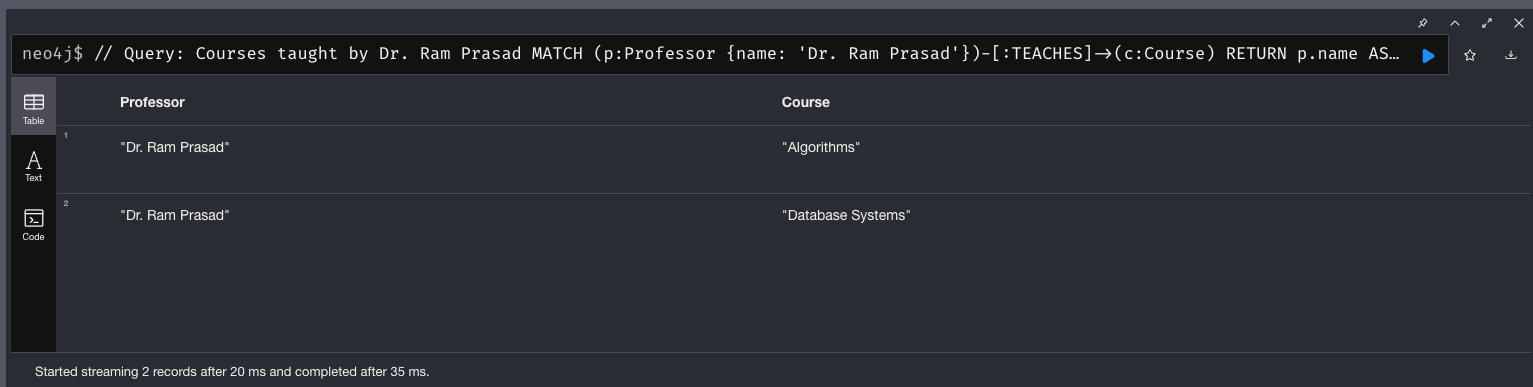
\includegraphics[width=0.8\textwidth]{task-3/screenshots/course-by-prof-ram-prasad.png}
  \caption{Query Result: Courses taught by Dr. Ram Prasad. This demonstrates filtered querying where specific node properties are used to constrain the search, showing only courses taught by a particular professor.}
  \label{fig:task3-courses-ram}
\end{figure}

\begin{figure}[H]
  \centering
  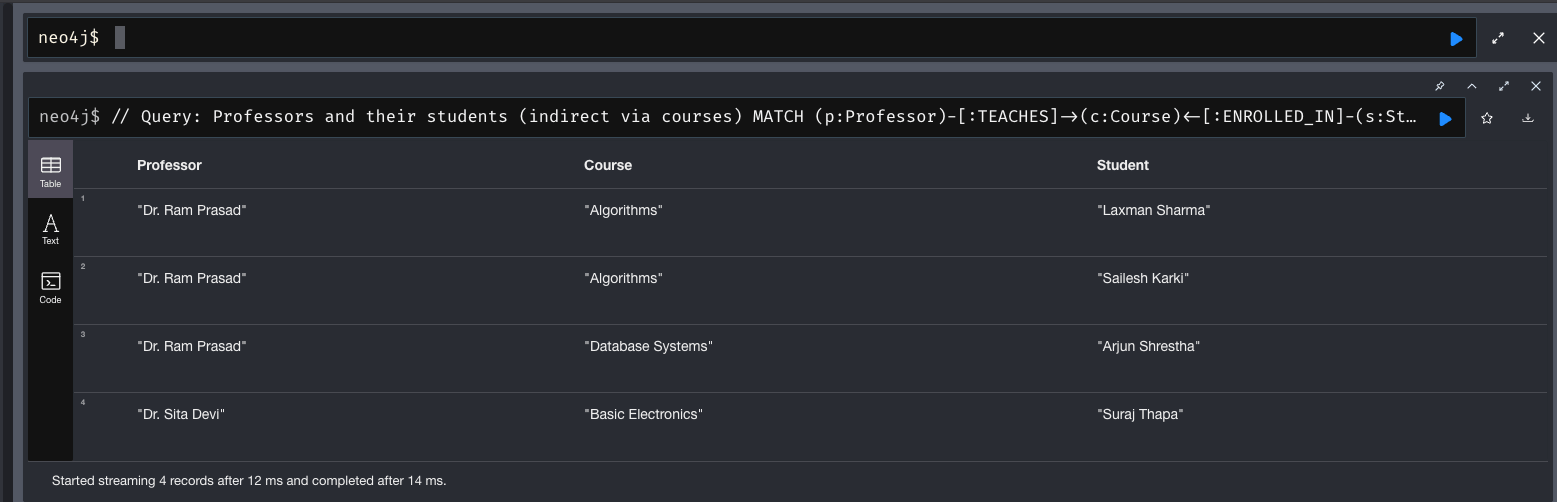
\includegraphics[width=0.8\textwidth]{task-3/screenshots/prof-and-their-students.png}
  \caption{Query Result: Professors and their students through courses. This screenshot illustrates complex graph traversal where the query follows multiple relationship paths (TEACHES and ENROLLED\_IN) to connect professors to their students indirectly through courses.}
  \label{fig:task3-prof-students}
\end{figure}

\begin{figure}[H]
  \centering
  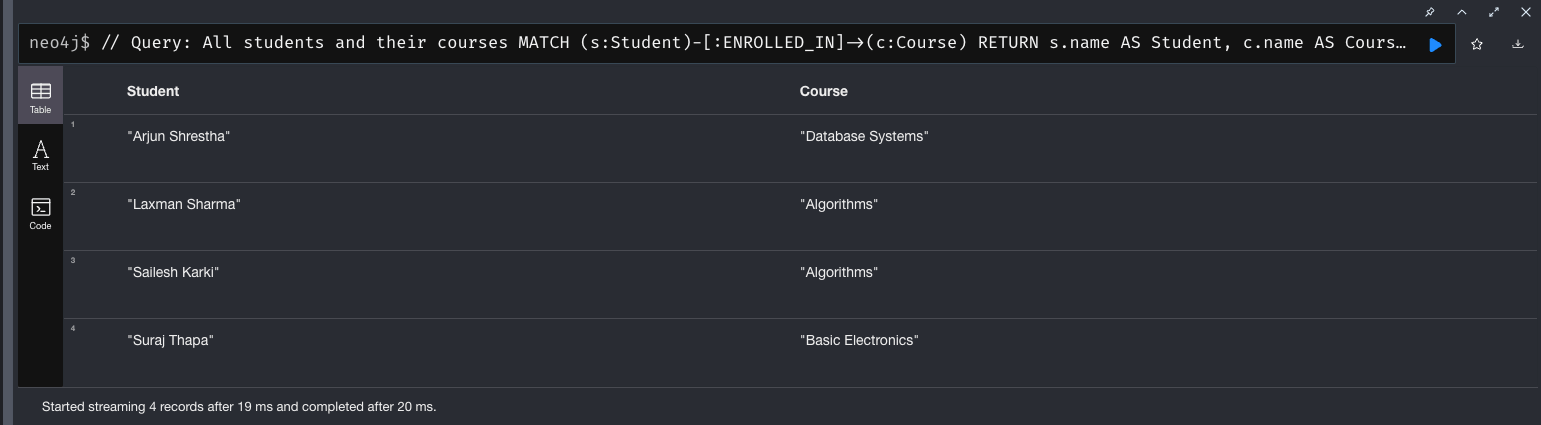
\includegraphics[width=0.8\textwidth]{task-3/screenshots/student-and-their-courses.png}
  \caption{Query Result: All students and their enrolled courses. This shows the reverse traversal of the ENROLLED\_IN relationship, listing students and the courses they are taking.}
  \label{fig:task3-student-courses}
\end{figure}

\begin{figure}[H]
  \centering
  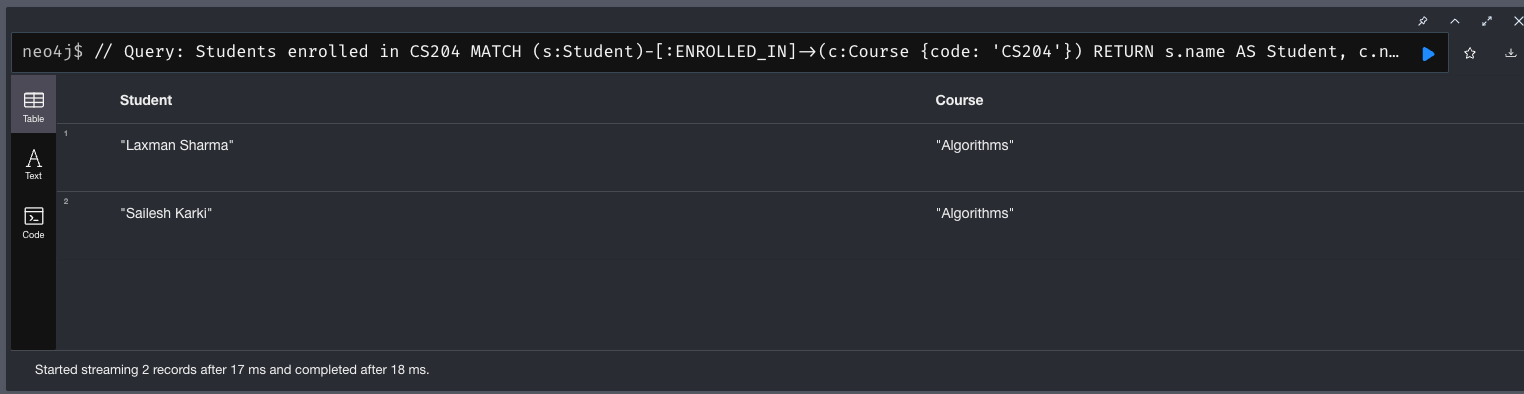
\includegraphics[width=0.8\textwidth]{task-3/screenshots/students-in-cs204.png}
  \caption{Query Result: Students enrolled in CS204 (Algorithms). This demonstrates property-based filtering at the course level, showing how to find all students enrolled in a specific course using course codes.}
  \label{fig:task3-students-cs204}
\end{figure}

\begin{figure}[H]
  \centering
  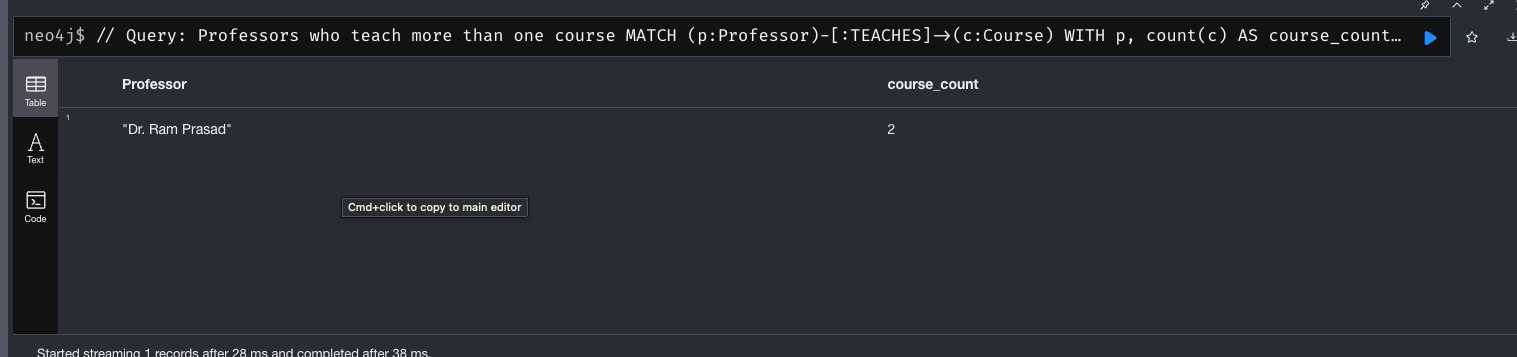
\includegraphics[width=0.8\textwidth]{task-3/screenshots/who-teaches-more-than-one-course.png}
  \caption{Query Result: Professors teaching multiple courses. This screenshot shows an aggregation query that counts relationships per professor and filters results, demonstrating Neo4j's capability for analytical queries.}
  \label{fig:task3-multi-course-prof}
\end{figure}

\begin{figure}[H]
  \centering
  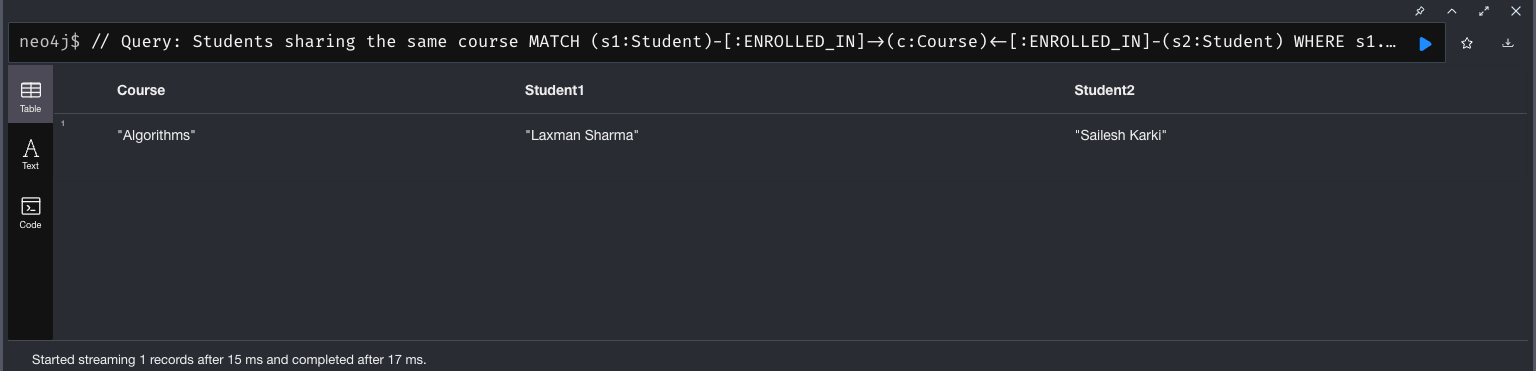
\includegraphics[width=0.8\textwidth]{task-3/screenshots/student-doing-same-course.png}
  \caption{Query Result: Students enrolled in the same course. This demonstrates a more complex pattern matching query that finds pairs of students connected through the same course, showcasing Neo4j's ability to discover indirect relationships.}
  \label{fig:task3-same-course}
\end{figure}

\section{Redis Key-Value Store Screenshots}

The following screenshots document the implementation and operation of Redis for key-value store operations, session management with TTL, and visitor tracking using atomic increment operations.

\begin{figure}[H]
  \centering
  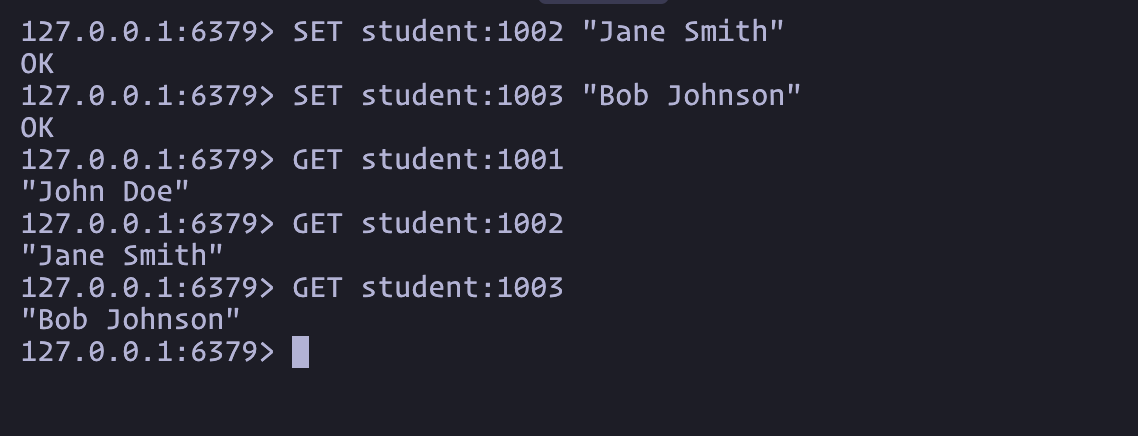
\includegraphics[width=0.8\textwidth]{task-4/screenshots/basic-set-get-operations.png}
  \caption{Basic Redis String Operations: SET and GET commands demonstration. This shows simple key-value pair storage and retrieval operations, which form the foundation of Redis data manipulation.}
  \label{fig:basic-set-get}
\end{figure}

\begin{figure}[H]
  \centering
  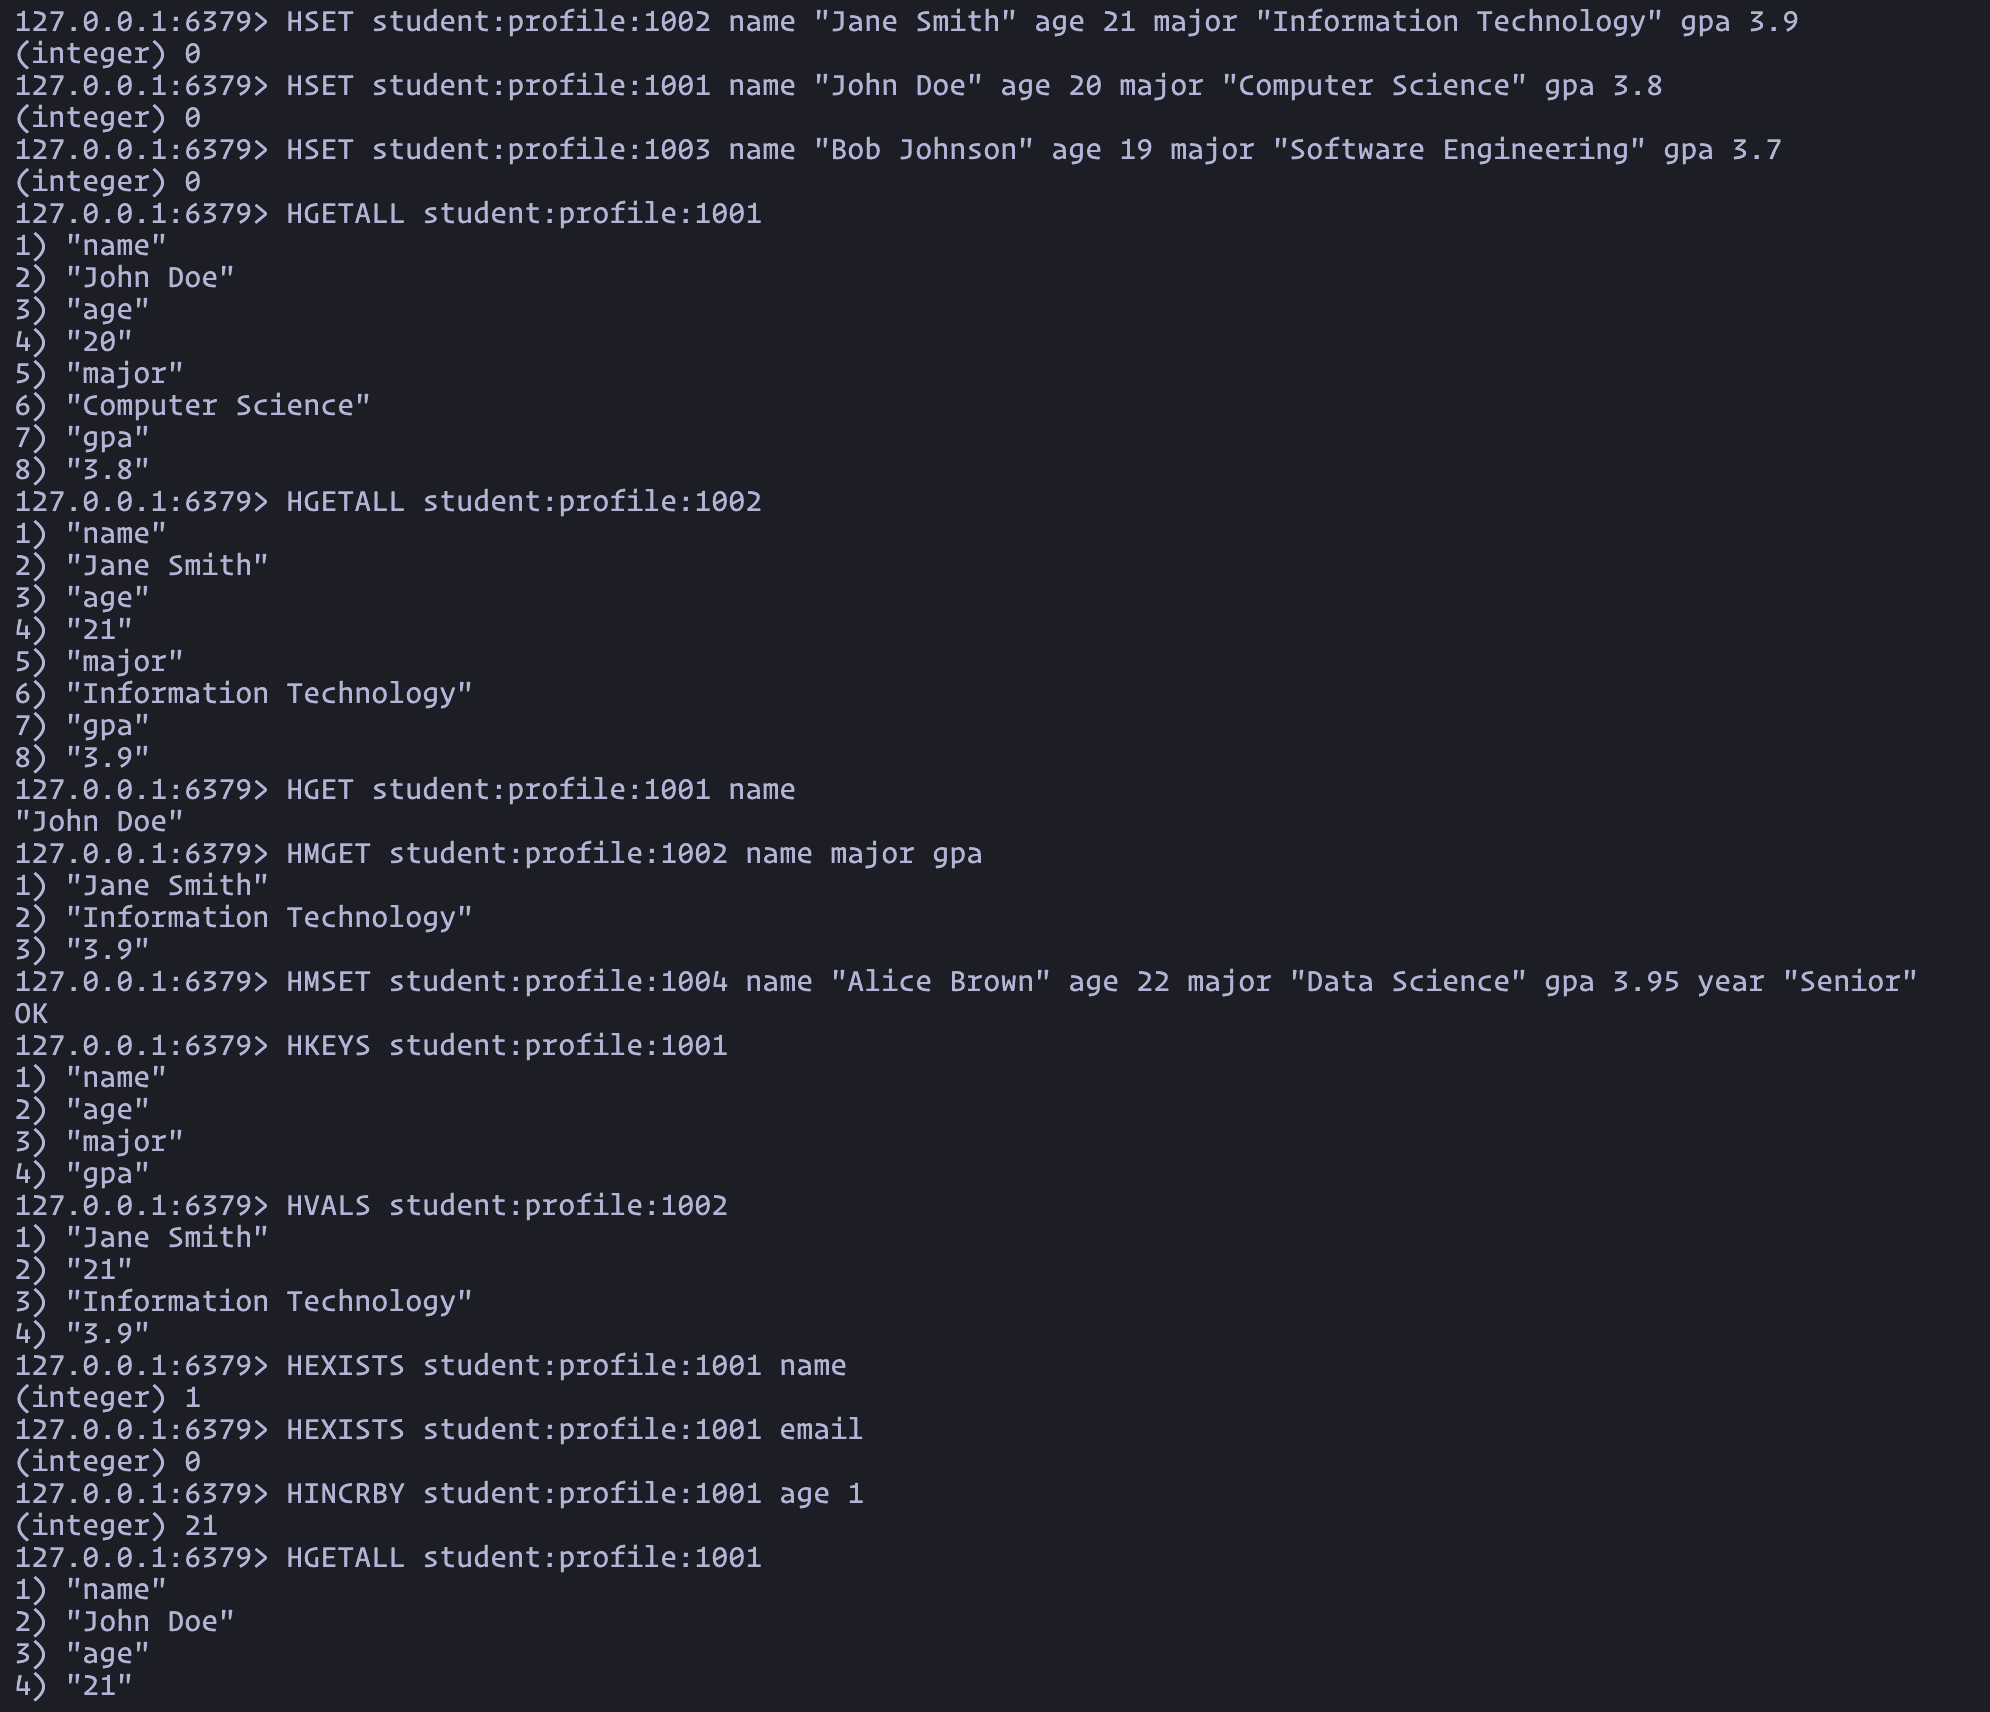
\includegraphics[width=0.8\textwidth]{task-4/screenshots/hash-operations.png}
  \caption{Redis Hash Operations: HSET, HGETALL, HGET, and related hash commands. This demonstrates Redis's ability to store structured data using field-value pairs within a single key, ideal for object representation.}
  \label{fig:hash-operations}
\end{figure}

\begin{figure}[H]
  \centering
  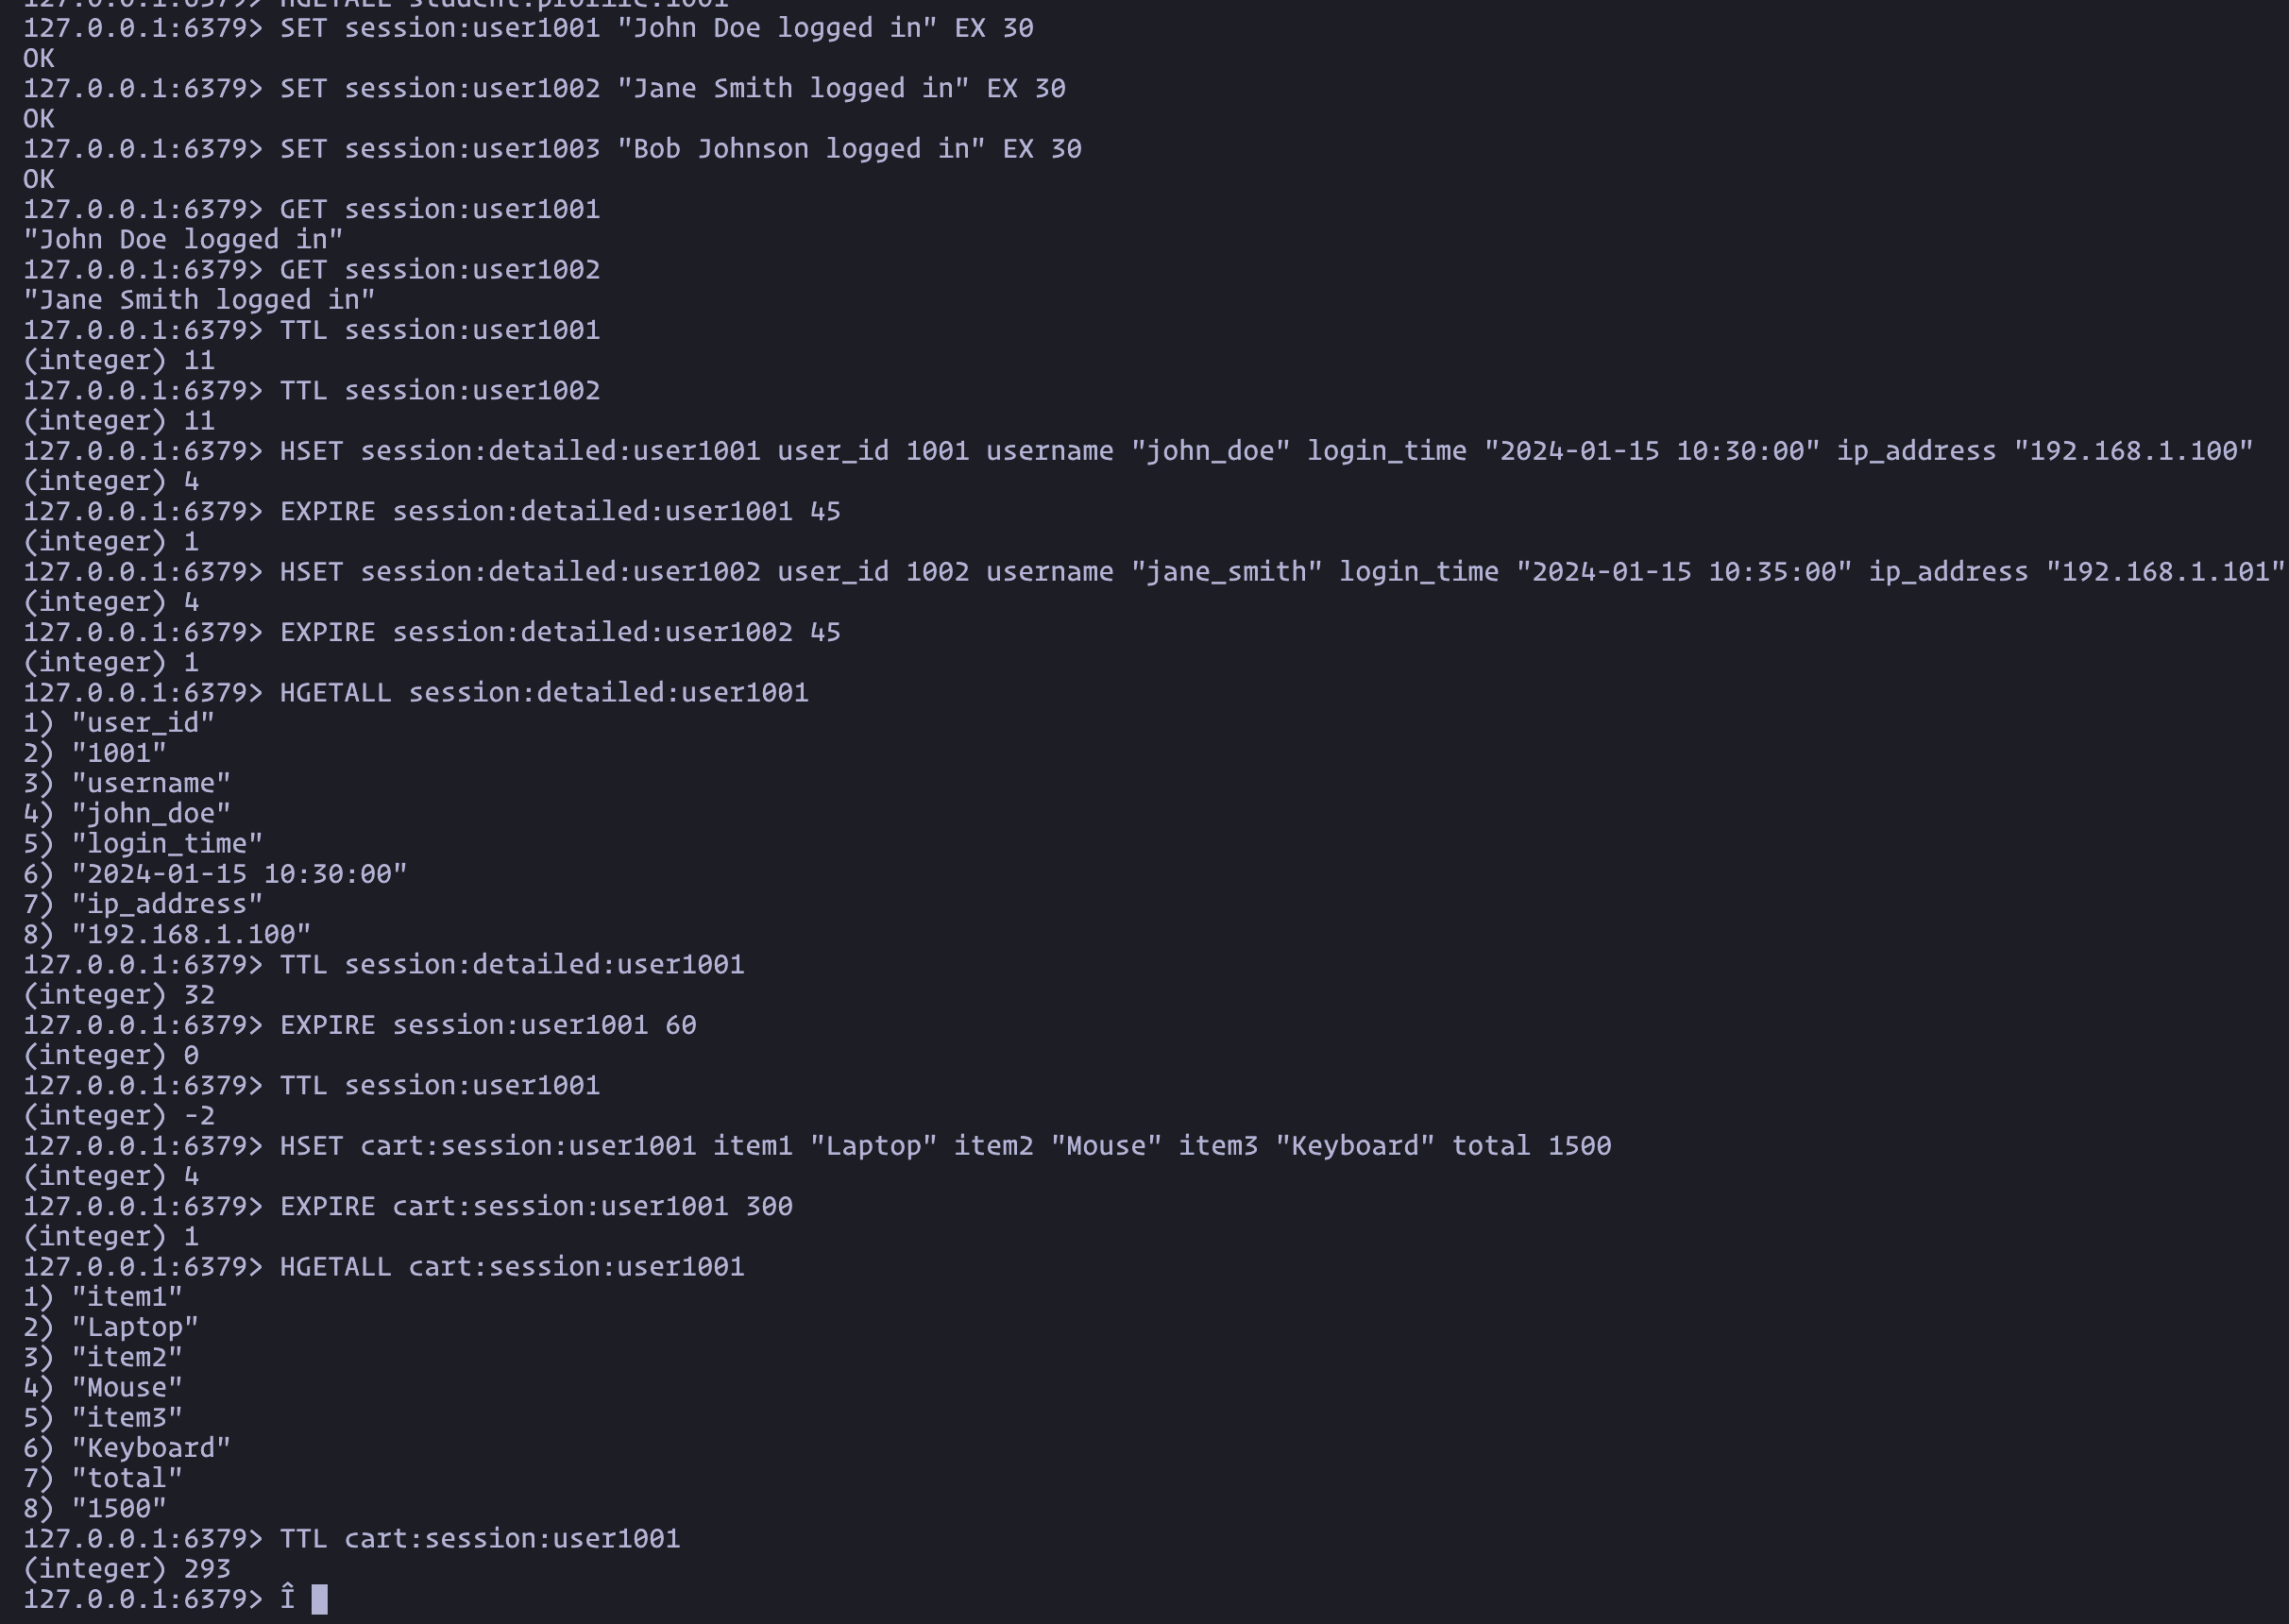
\includegraphics[width=0.8\textwidth]{task-4/screenshots/session-details.png}
  \caption{Session Management with TTL: Creating user sessions with automatic expiration. This shows Redis's TTL functionality for managing temporary data like user sessions, shopping carts, and cached content.}
  \label{fig:session-details}
\end{figure}

\begin{figure}[H]
  \centering
  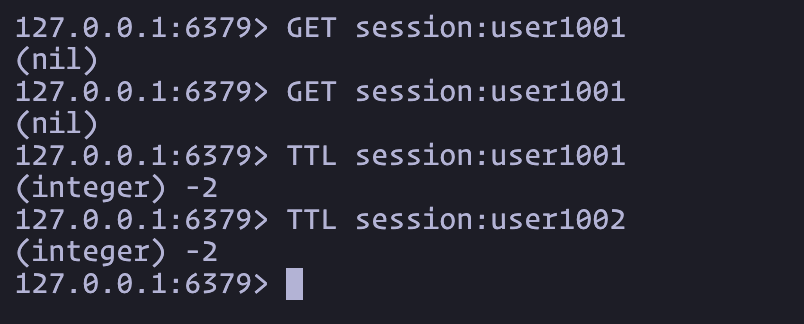
\includegraphics[width=0.8\textwidth]{task-4/screenshots/session-expiration.png}
  \caption{Session Expiration Results: Demonstrating automatic key deletion after TTL expires. This shows how Redis automatically cleans up expired keys, returning nil for expired sessions and -2 for TTL checks.}
  \label{fig:session-expiration}
\end{figure}

\begin{figure}[H]
  \centering
  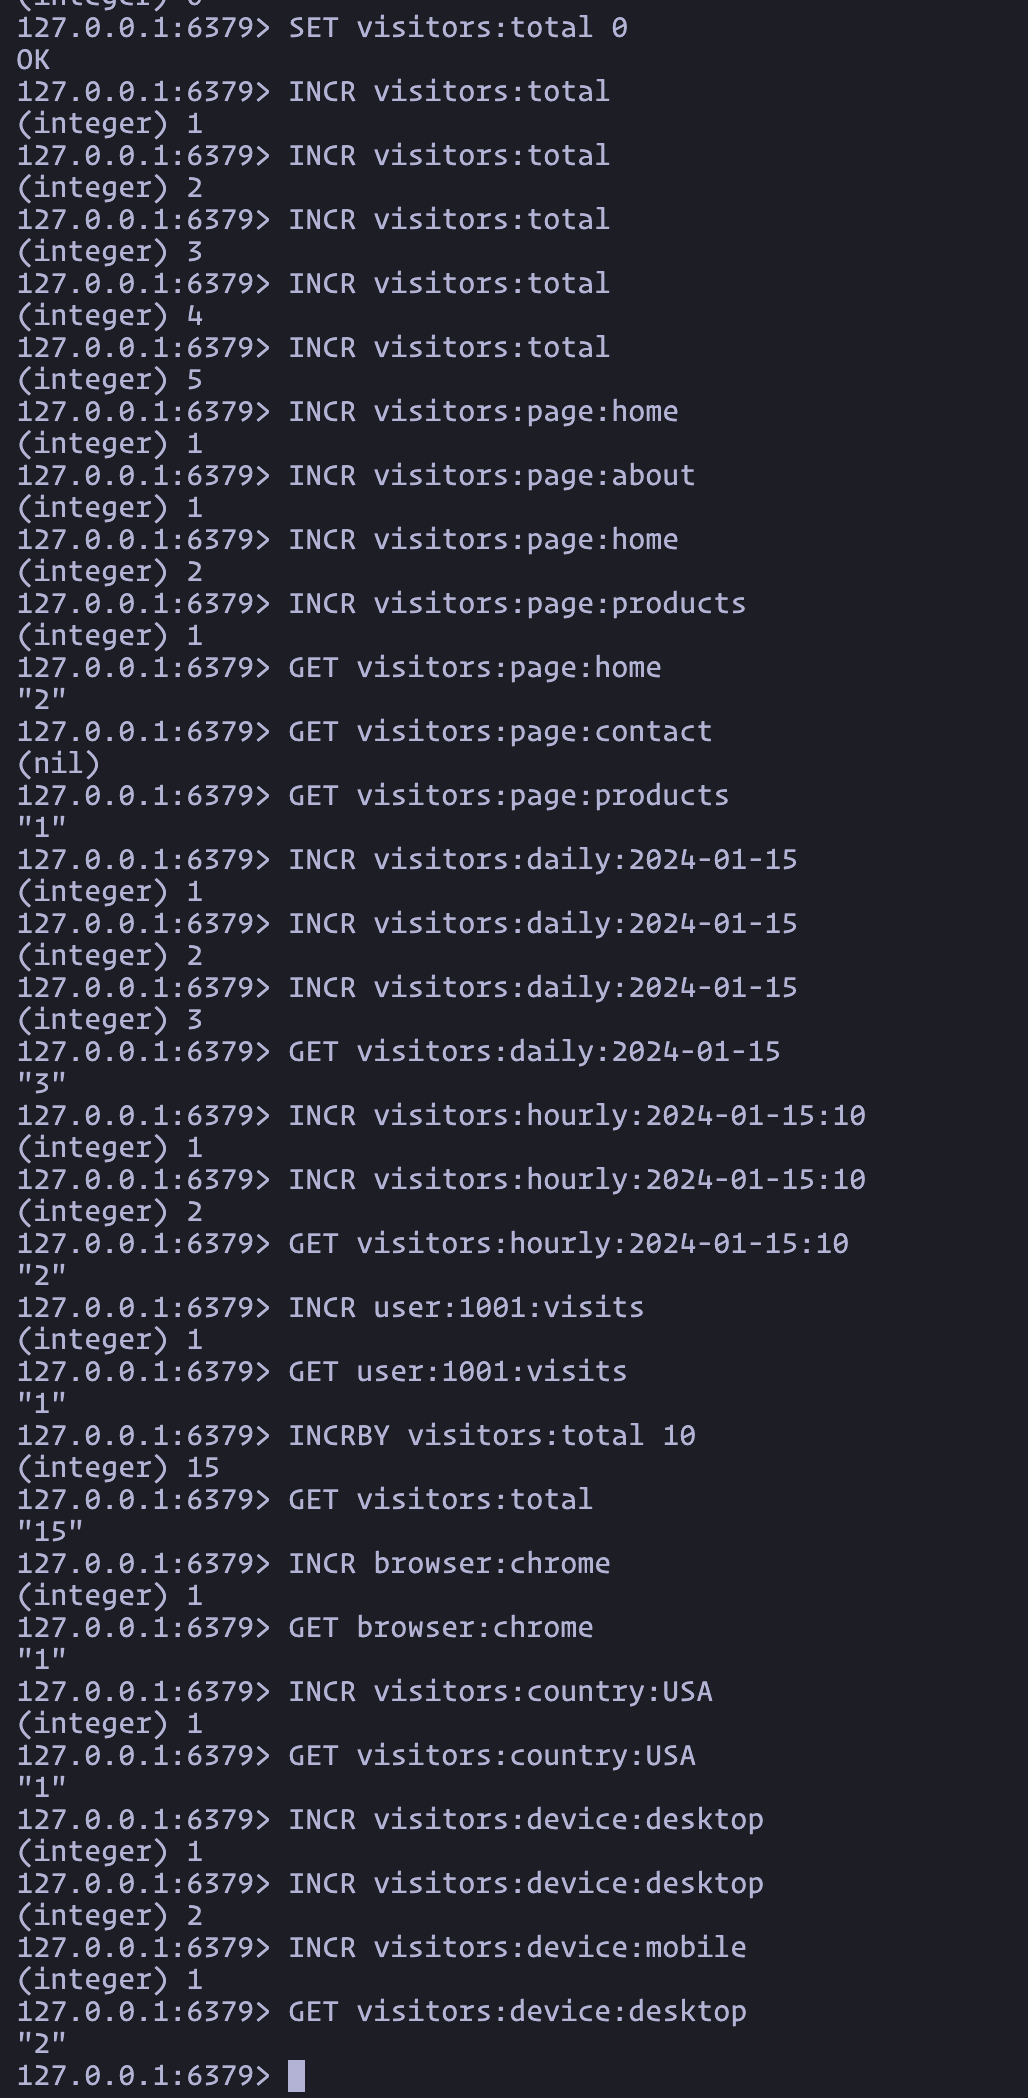
\includegraphics[width=0.8\textwidth]{task-4/screenshots/visitor-tracking.png}
  \caption{Visitor Tracking with INCR Operations: Atomic increment operations for analytics and counting. This demonstrates Redis's atomic counter capabilities for page views, user visits, browser tracking, and other analytics metrics.}
  \label{fig:visitor-tracking}
\end{figure}

\section{CockroachDB Distributed SQL Screenshots}

The following screenshots document the implementation and operation of CockroachDB for distributed SQL operations, demonstrating ACID transactions, concurrent transfers, and banking operations.

\subsection*{Database Setup and Schema Creation}

\begin{figure}[H]
  \centering
  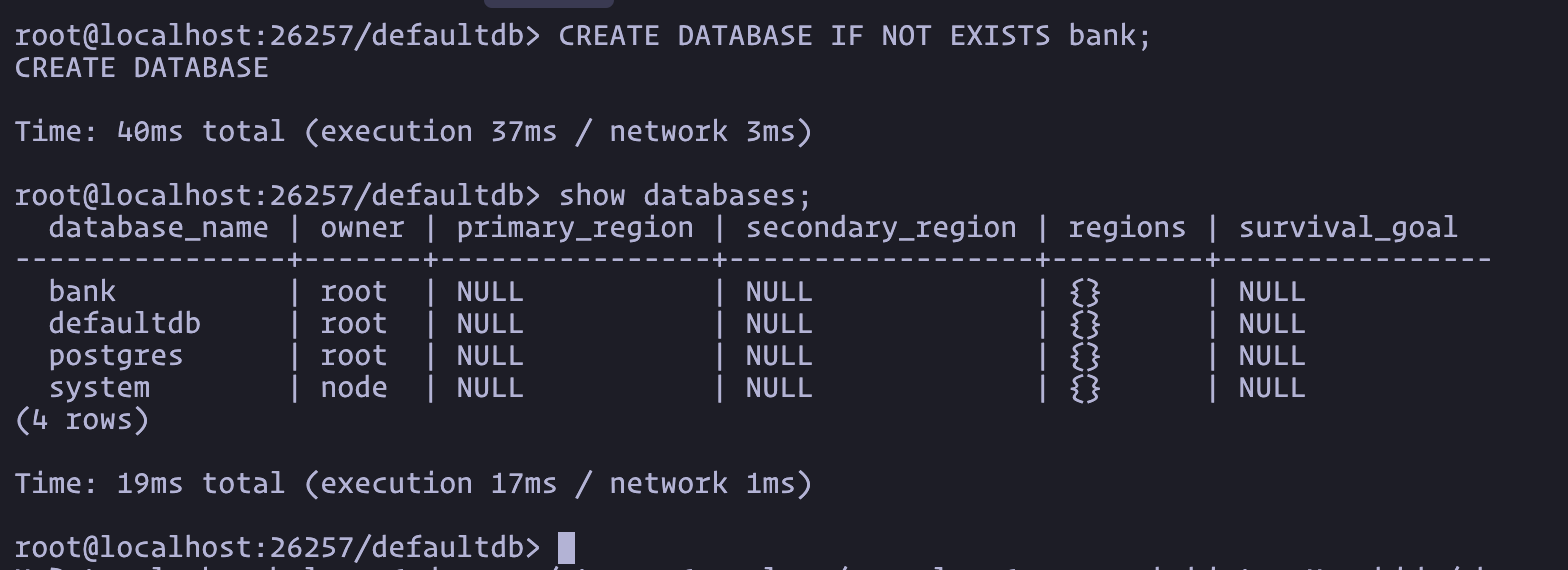
\includegraphics[width=0.8\textwidth]{task-5/screenshots/create-db.png}
  \caption{Database Creation Process: Terminal output showing the successful creation of the \texttt{bank} database in CockroachDB. This demonstrates the initial setup phase where the database environment is established for the banking application.}
  \label{fig:task5-create-db}
\end{figure}

\begin{figure}[H]
  \centering
  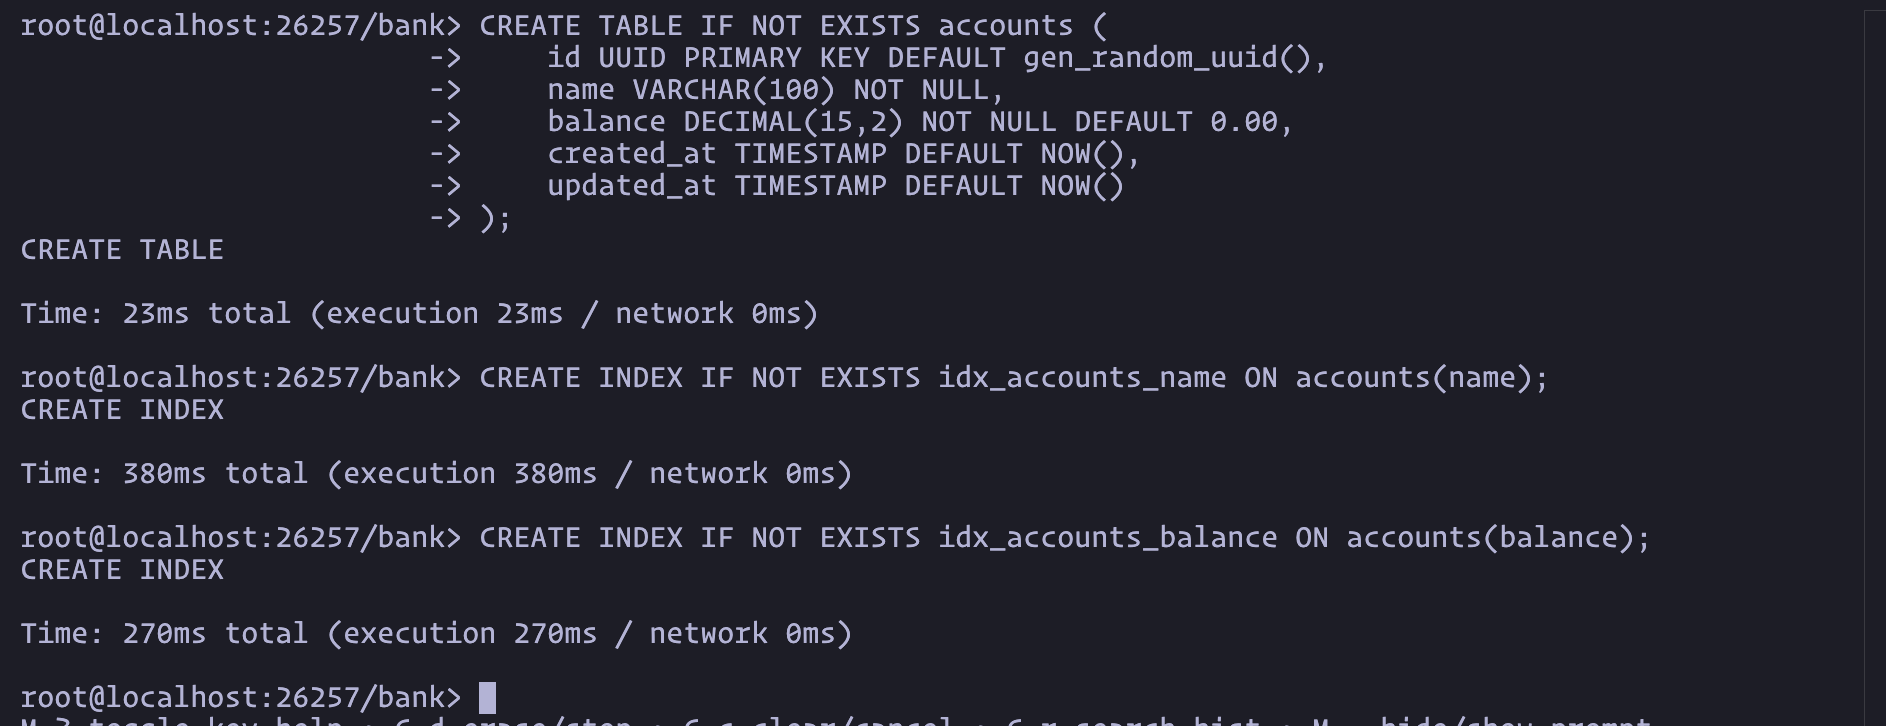
\includegraphics[width=0.8\textwidth]{task-5/screenshots/create-table.png}
  \caption{Table Structure Creation: Screenshot displaying the creation of the \texttt{accounts} table with UUID primary key, proper data types, and indexes. This shows the schema design optimized for distributed transactions and ACID compliance.}
  \label{fig:task5-create-table}
\end{figure}

\begin{figure}[H]
  \centering
  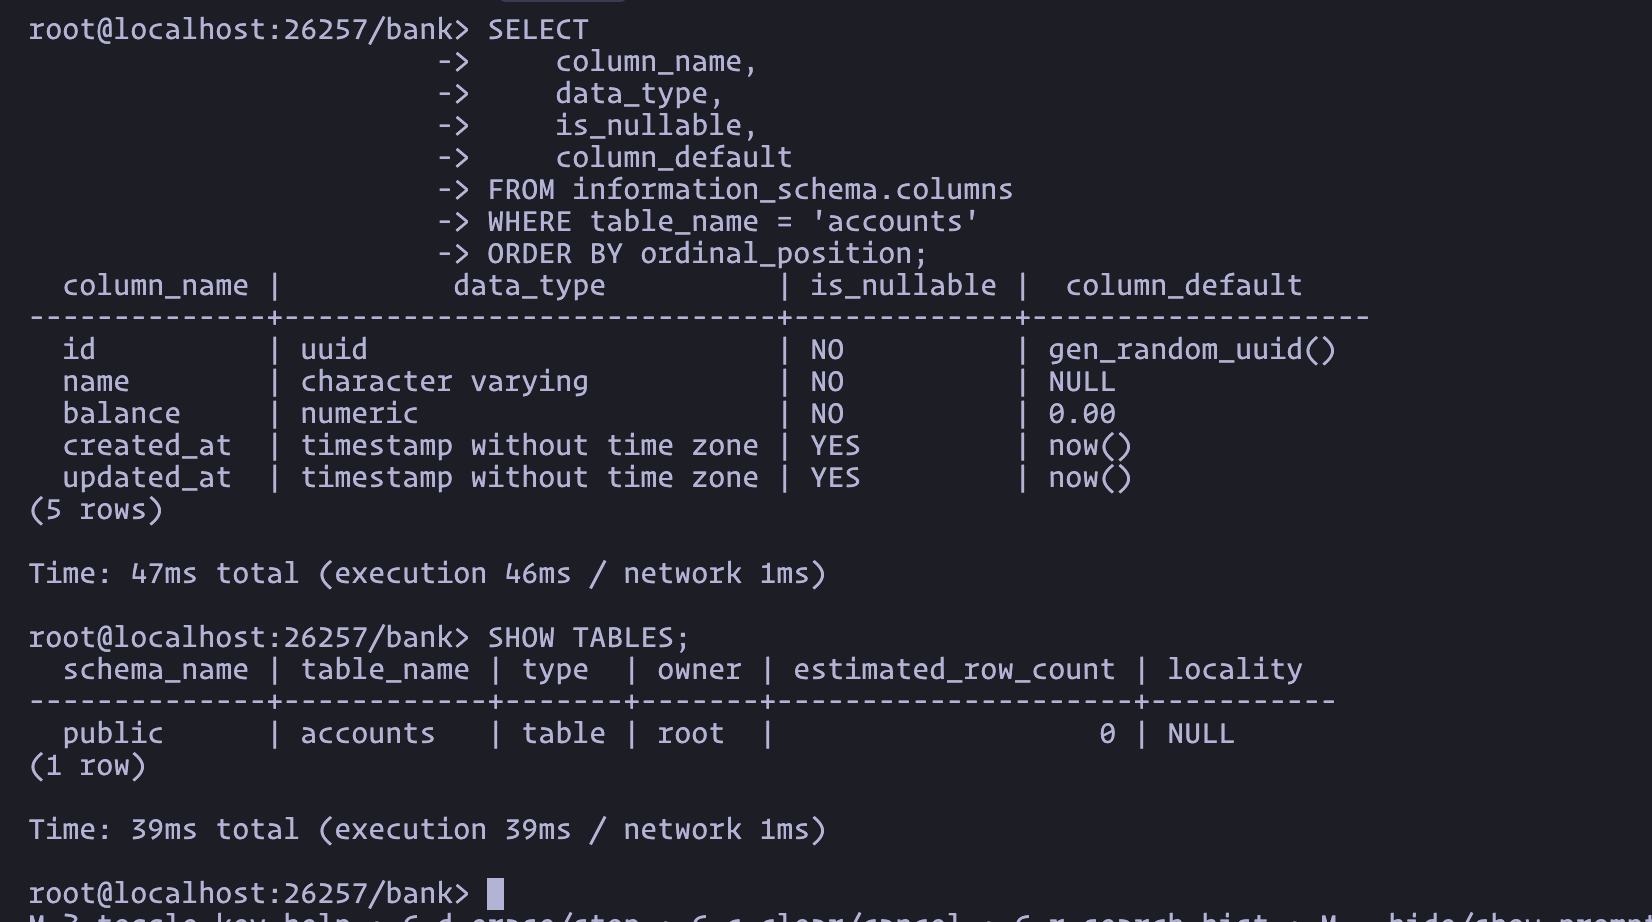
\includegraphics[width=0.8\textwidth]{task-5/screenshots/table-structure.png}
  \caption{Table Structure Display: Detailed view of the accounts table schema showing column names, data types, nullability, and default values. This demonstrates the complete table structure created for the banking application.}
  \label{fig:task5-table-structure}
\end{figure}

\subsection*{Data Insertion and Verification}

\begin{figure}[H]
  \centering
  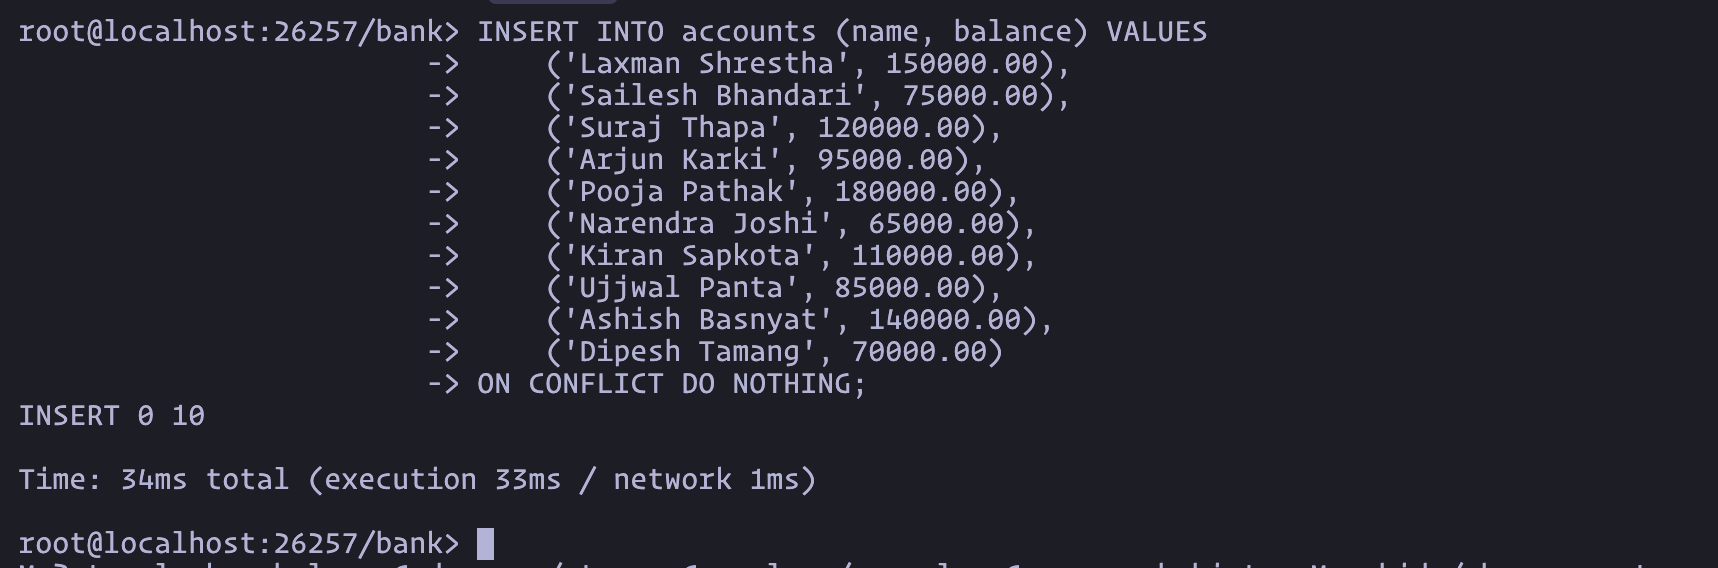
\includegraphics[width=0.8\textwidth]{task-5/screenshots/insert-balance.png}
  \caption{Account Data Insertion: Console output showing the successful insertion of 10 accounts with realistic balances. This demonstrates bulk data insertion with proper transaction handling in a distributed environment.}
  \label{fig:task5-insert-balance}
\end{figure}

\begin{figure}[H]
  \centering
  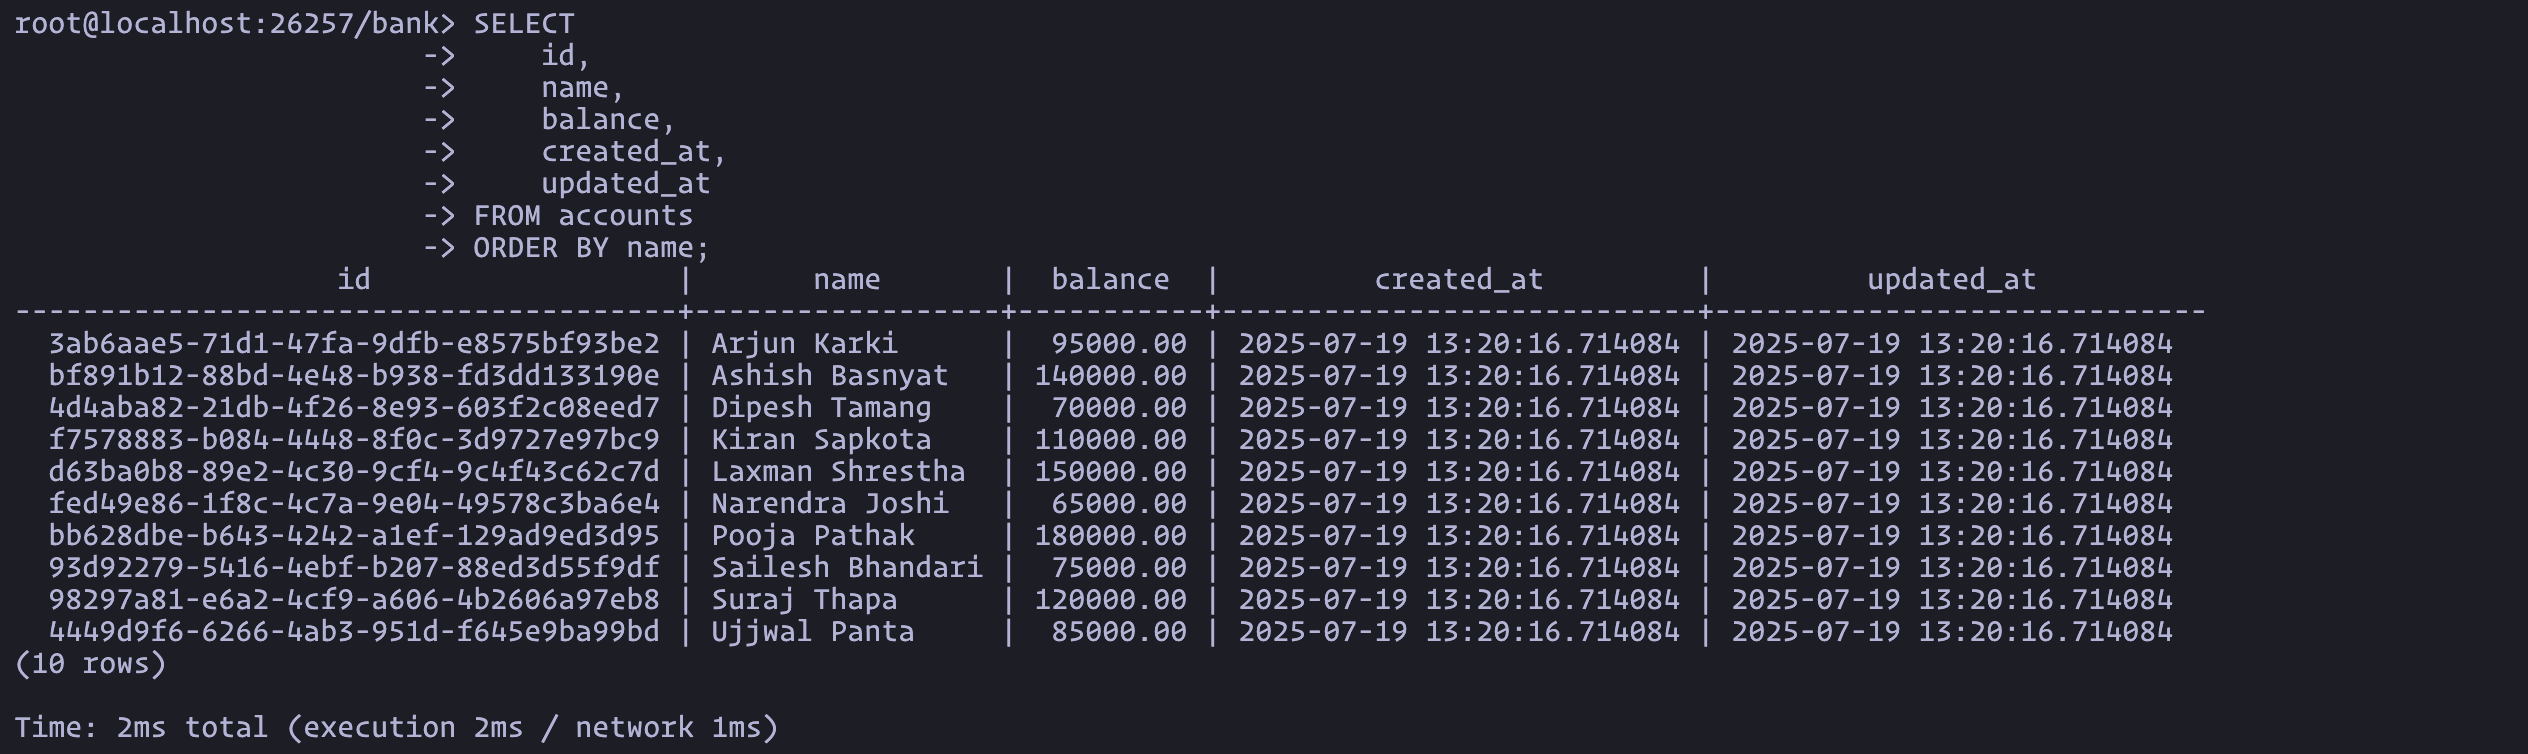
\includegraphics[width=0.8\textwidth]{task-5/screenshots/display-inserted-data.png}
  \caption{Inserted Accounts Display: Complete view of all inserted accounts showing generated UUIDs, names, balances, and timestamps. This verifies the data insertion process and demonstrates the distributed primary key generation.}
  \label{fig:task5-display-inserted}
\end{figure}

\begin{figure}[H]
  \centering
  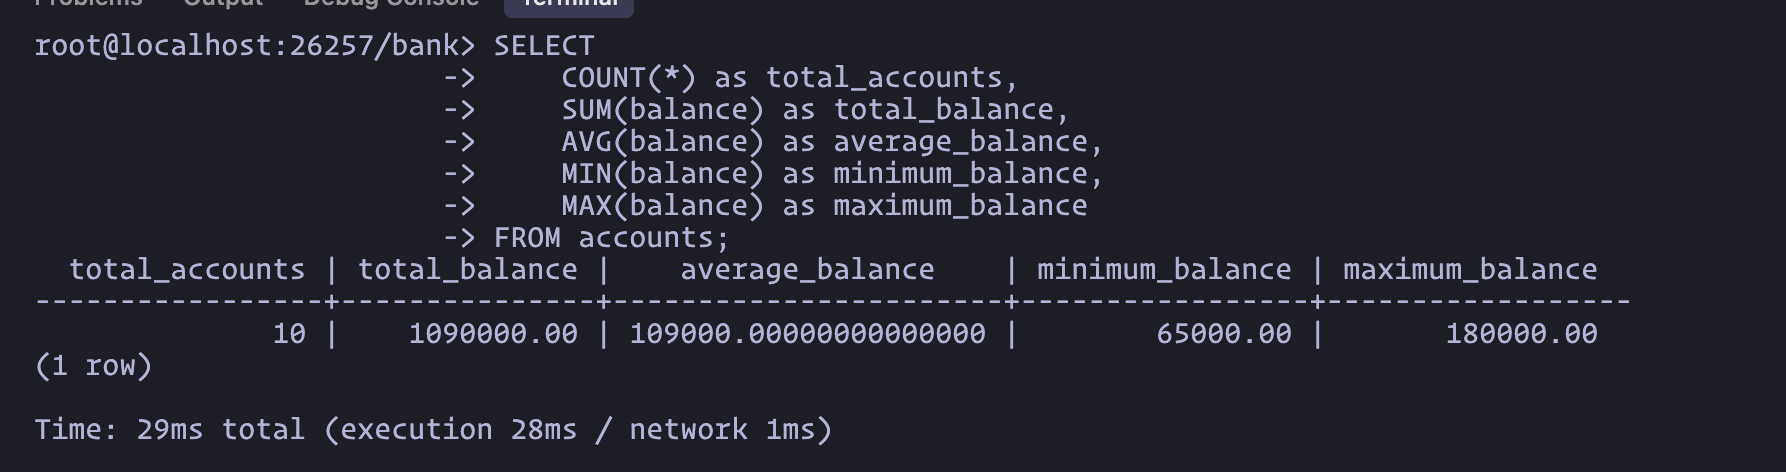
\includegraphics[width=0.8\textwidth]{task-5/screenshots/account-stats.png}
  \caption{Account Statistics After Insertion: Comprehensive statistics showing total accounts, total balance, average balance, and balance distribution after initial data insertion. This demonstrates the analytical capabilities of the distributed SQL database.}
  \label{fig:task5-account-stats}
\end{figure}

\subsection*{Transaction Operations}

\begin{figure}[H]
  \centering
  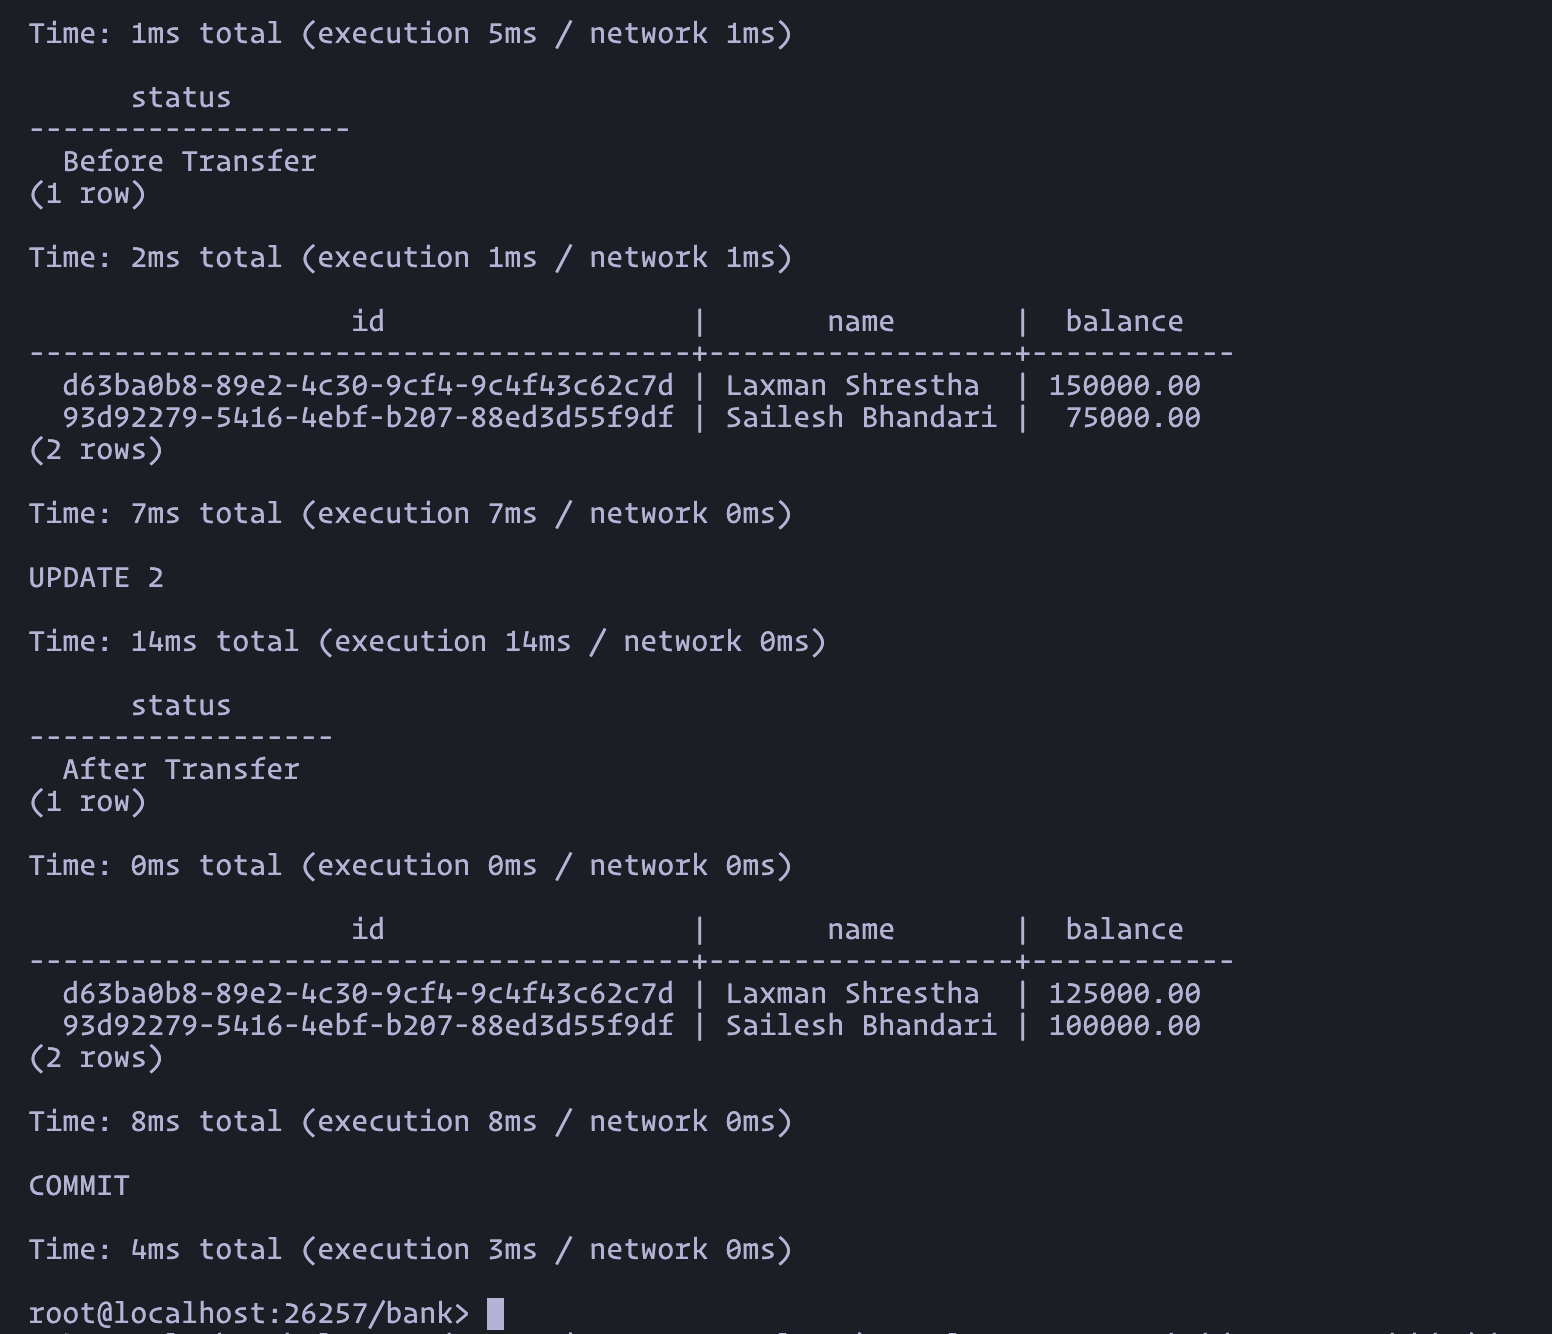
\includegraphics[width=0.8\textwidth]{task-5/screenshots/single-transfer.png}
  \caption{Single Transfer Transaction: Demonstration of ACID-compliant transfer between two accounts. The screenshot shows the before and after states of the accounts involved in the transfer, proving atomicity and consistency of the transaction.}
  \label{fig:task5-single-transfer}
\end{figure}

\begin{figure}[H]
  \centering
  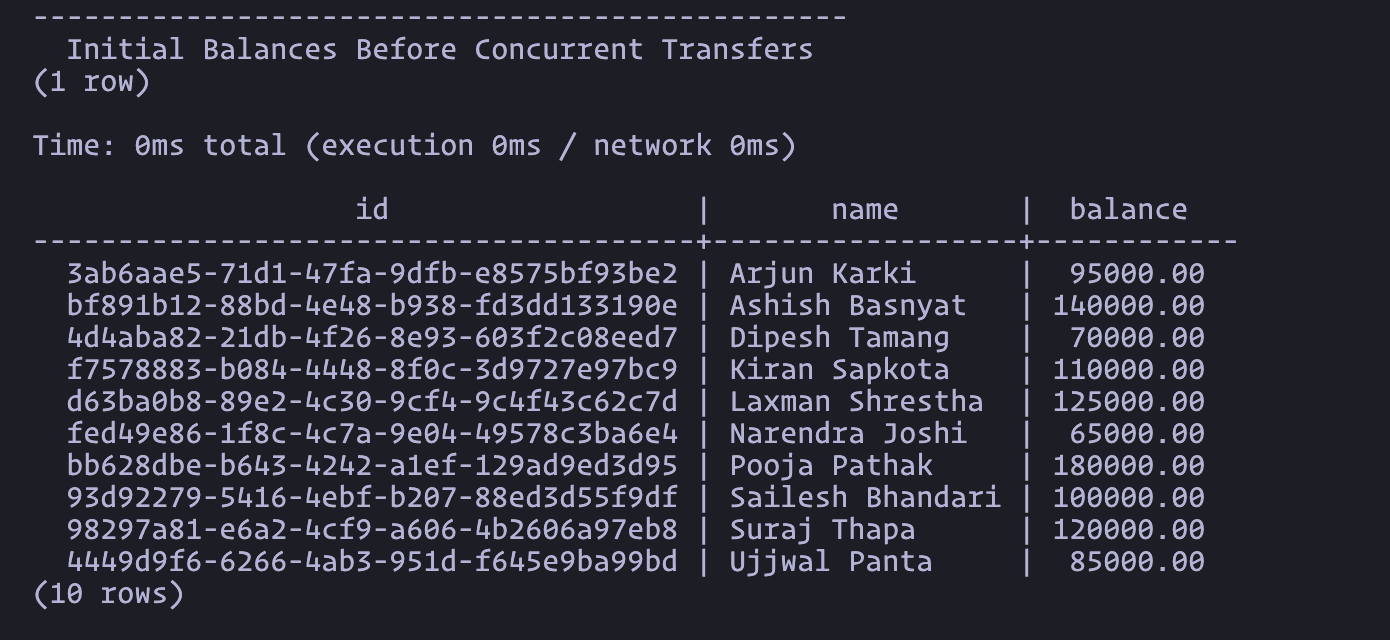
\includegraphics[width=0.8\textwidth]{task-5/screenshots/initial-before-concurrent.png}
  \caption{Initial Balances Before Concurrent Transfers: Account balances before executing multiple concurrent transfer operations. This establishes the baseline state for demonstrating CockroachDB's concurrent transaction handling capabilities.}
  \label{fig:task5-initial-before-concurrent}
\end{figure}

\begin{figure}[H]
  \centering
  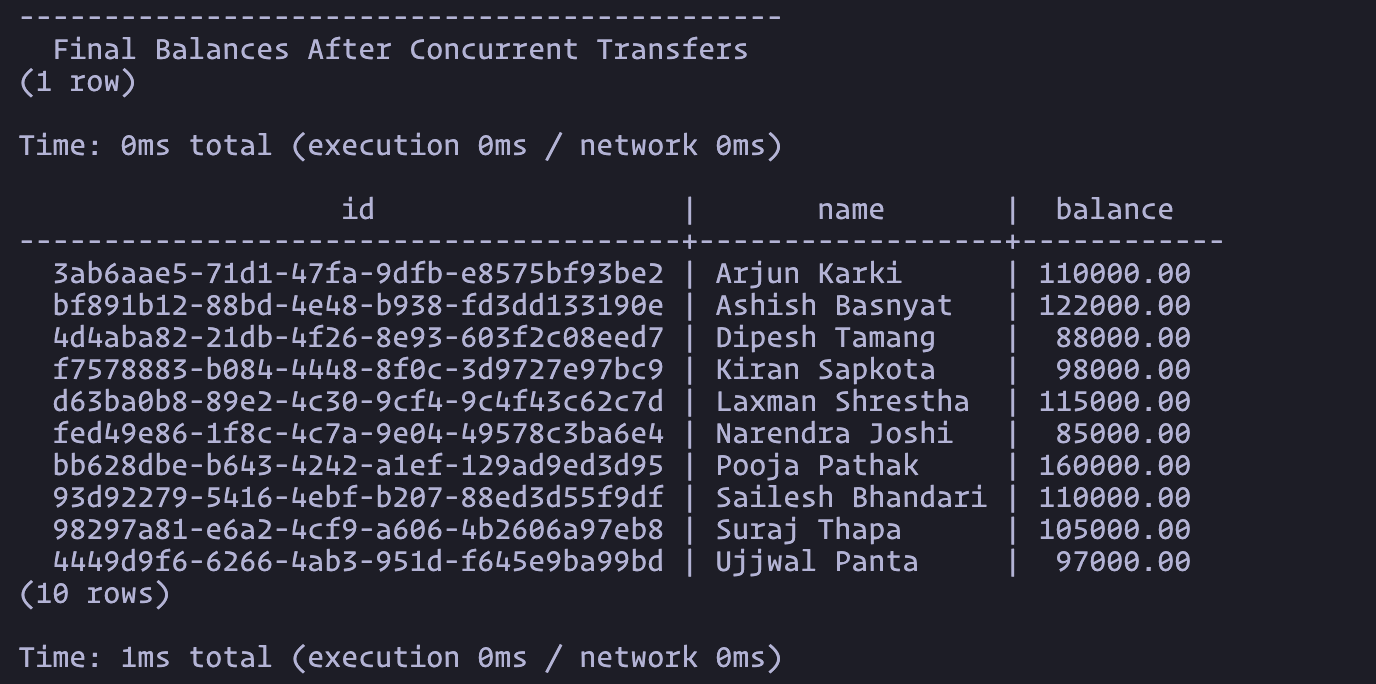
\includegraphics[width=0.8\textwidth]{task-5/screenshots/final-after-concurrent.png}
  \caption{Final Balances After Concurrent Transfers: Account balances after all concurrent transfers complete successfully. This demonstrates CockroachDB's ability to handle multiple simultaneous transactions while maintaining ACID compliance and data consistency.}
  \label{fig:task5-final-after-concurrent}
\end{figure}

\subsection*{Analytics and Reporting}

\begin{figure}[H]
  \centering
  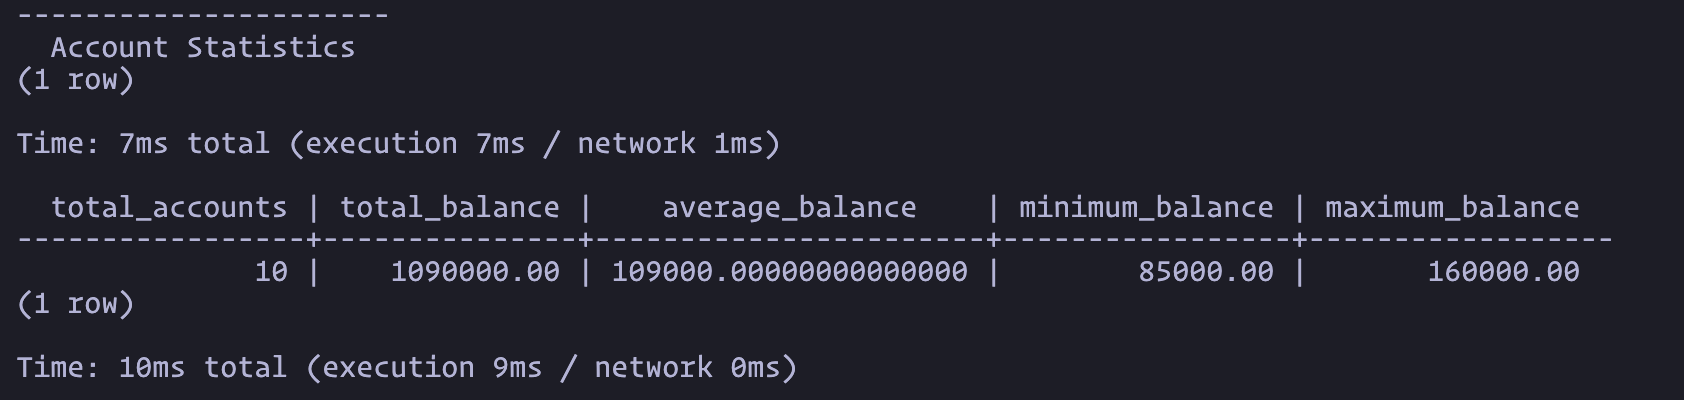
\includegraphics[width=0.8\textwidth]{task-5/screenshots/account-stats-after-txns.png}
  \caption{Account Statistics After Transactions: Comprehensive statistics showing total accounts, total balance, average balance, and balance distribution. This demonstrates the analytical capabilities of the distributed SQL database for financial reporting.}
  \label{fig:task5-account-stats-after-txns}
\end{figure}

\begin{figure}[H]
  \centering
  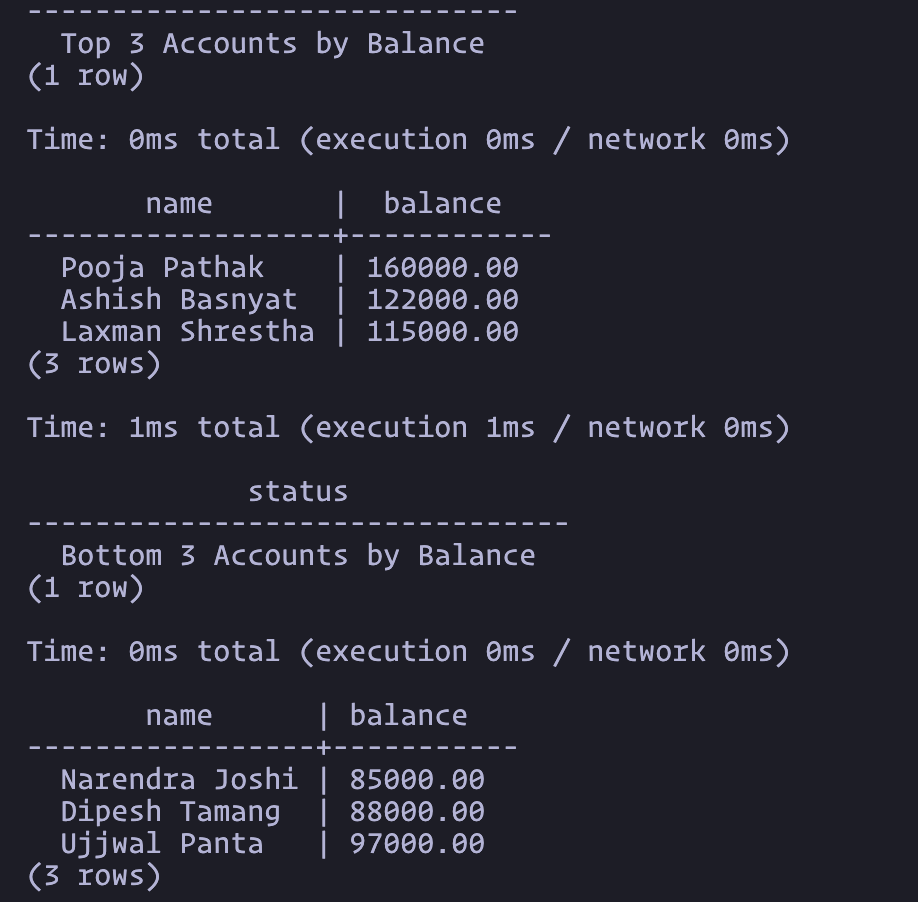
\includegraphics[width=0.8\textwidth]{task-5/screenshots/top-bottom-accounts.png}
  \caption{Top and Bottom Accounts by Balance: Ranking analysis showing accounts with highest and lowest balances. This demonstrates advanced querying capabilities for financial analysis and customer segmentation in the banking application.}
  \label{fig:task5-top-bottom-accounts}
\end{figure}

\begin{figure}[H]
  \centering
  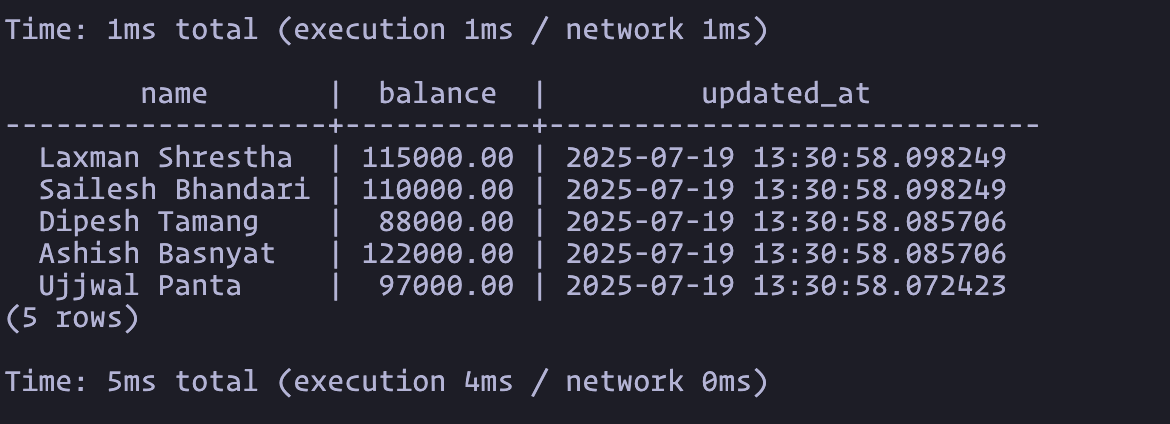
\includegraphics[width=0.8\textwidth]{task-5/screenshots/recently-updated-accounts.png}
  \caption{Recently Updated Accounts: Audit trail showing accounts that have been recently modified, including their current balances and update timestamps. This demonstrates the audit and monitoring capabilities essential for banking applications.}
  \label{fig:task5-recently-updated-accounts}
\end{figure}

\begin{figure}[H]
  \centering
  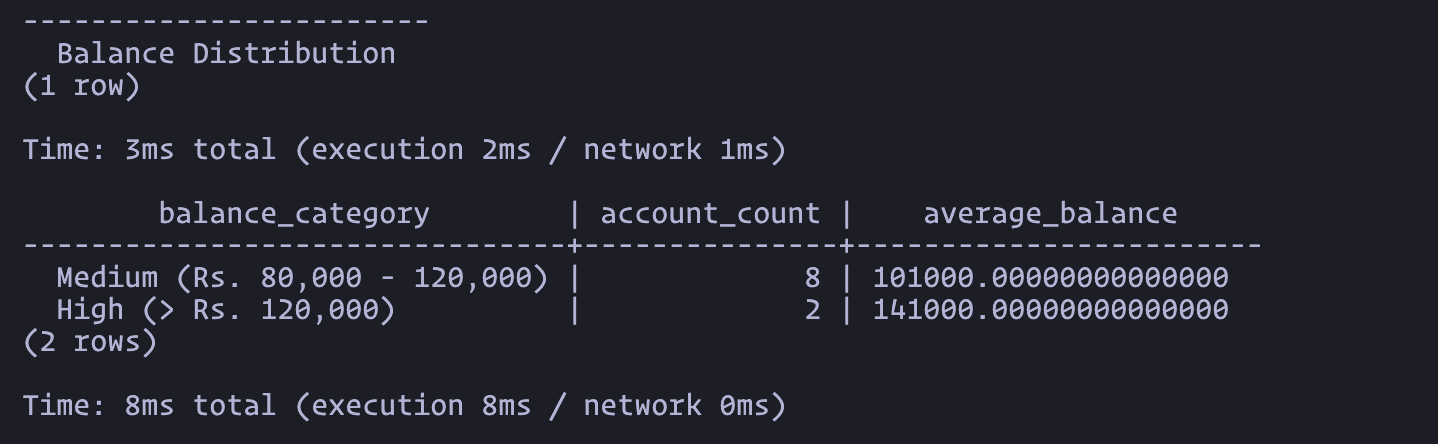
\includegraphics[width=0.8\textwidth]{task-5/screenshots/balance-distribution.png}
  \caption{Balance Distribution Analysis: Categorization of accounts by balance ranges (Low, Medium, High) with count and average balance for each category. This demonstrates advanced analytical capabilities for customer segmentation and financial reporting.}
  \label{fig:task5-balance-distribution}
\end{figure}